% Main LaTeX document for the RSS'09 Booklet
\documentclass[9pt, twoside, openany]{extbook}


\usepackage{ifthen}

%define to switch between different flavours:
%\def \targetoutput {print}  %generate for printing (no colored hyperlinks, pages are all upright)
%\def \targetoutput {usbstick} %optimized for screen viewing, pre-rotated landscape pages, links to local files
\def \targetoutput {online}

\usepackage{fleqn}
%\usepackage{latexpackages/my}
\usepackage{times}
\usepackage[normalem]{ulem}
\usepackage{eurosym}
\usepackage{setspace}
\usepackage{graphicx}
\usepackage{epstopdf}
%\usepackage{epsfig}
%\newcommand{\denselist}{\itemsep -3pt\topsep 0pt\partopsep 0pt\parsep 0pt}

\usepackage[a4paper,top=3cm, left=1.5cm, right=1.5cm, bottom=2.5cm, headsep=1.5cm, footskip=8mm]{geometry}
\setlength{\headheight}{34pt} %adjust headheight to suppress warnings

%\pdfoutput=0
\usepackage{wrapfig,graphicx}
\usepackage{hyperref}


\ifthenelse{\equal{\targetoutput}{print}}{
  \hypersetup{bookmarksopen,bookmarksnumbered,
  pdfpagemode=UseOutlines,
  colorlinks=true,
  linkcolor=black,
  anchorcolor=black,
  citecolor=black,
  filecolor=black,
  menucolor=black,
  urlcolor=black,
  debug=true
  }
}{
  \hypersetup{bookmarksopen,bookmarksnumbered,
  pdfpagemode=UseOutlines,
  colorlinks=true,
  linkcolor=blue,
  anchorcolor=blue,
  citecolor=blue,
  filecolor=blue,
  menucolor=blue,
  urlcolor=blue,
  }
}

\usepackage[utf8]{inputenc}
\usepackage[english]{babel}
\usepackage{array}
\usepackage{wrapfig}

\DeclareGraphicsExtensions{.pdf,.jpg, .png}

\usepackage[usenames,dvipsnames]{xcolor}
%\definecolor{RSSorange}{HTML}{F2531B}
\definecolor{RSSblue}{HTML}{002654}

%\usepackage[table]{xcolor}
\usepackage{tabularx}
\newboolean{include-notes}
\setboolean{include-notes}{true}

% http://en.wikibooks.org/wiki/LaTeX/Colors
\newcommand{\adnote}[1]{\ifthenelse{\boolean{include-notes}}%
 {\textcolor{LimeGreen}{\textbf{NOTE: #1}}}{}}

 
\ifthenelse{\equal{\targetoutput}{print}}{\usepackage{lscape}}{\usepackage{pdflscape}} %don't load pdflscape for print version

\ifthenelse{\equal{\targetoutput}{usbstick}}{
    \newcommand{\linkedfile}[2]{\href{#2}{#1}} %\linkedfile{this file}{path/filename}
}{
    \newcommand{\linkedfile}[2]{#1}
}


%these are for the fancy general schedule:
\usepackage{latexpackages/timetable}
\usepackage{colortbl}

 
\usepackage{array}
\newcolumntype{x}[1]{%
>{\centering\hspace{0pt}}p{#1}}%
\usepackage{multirow}

\usepackage{multicol}

\usepackage[explicit]{titlesec}
\usepackage{fancyhdr}
%\titleformat{\chapter}{\bf\huge\center}{\thechapter}{0.2cm}{}
%don't print chapter name at the chapter beginning:
\titleformat{\chapter}{}{ }{0pt}{}
\titlespacing{\chapter}
   {0cm}% left
   {0cm}% before
   {0cm}% after

\titleformat{\section}{\sf \LARGE}{\thesection}{1em}{#1}
\titleformat{\subsection}{\sf \Large}{\thesubsection}{1em}{#1}
%\titlespacing{command}{left spacing}{before spacing}{after spacing}[right]
\titlespacing{\section} {0pt}{0.5ex plus 3ex}{0.8ex}



\fancypagestyle{default}{%
    \fancyhf{}
    \fancyhead[C]{}
    \fancyhead[RO,LE]{
\includegraphics[height=1.0cm]{local_img/logo.png}}
    \fancyhead[RE,LO]{\sf\LARGE \leftmark}
    %footer
    \fancyfoot[RO,LE]{\sf\thepage}
    \fancyfoot[RE,LO]{}
    \fancyfoot[C]{\sf2014 Berkeley, USA}
}
\fancypagestyle{plain}{}

\fancypagestyle{front}{%
    \fancyhf{}
    \fancyhead[C]{}
    \fancyhead[RO,LE]{
\includegraphics[height=1.0cm]{local_img/logo.png}}
    %footer
    \fancyfoot[RO,LE]{\sf\thepage}
    \fancyfoot[RE,LO]{}
    \fancyfoot[C]{\sf2014 Berkeley, USA}
} 


\setcounter{secnumdepth}{-2} %suppress all numbering, even chapter and part

\widowpenalty=300
\clubpenalty=300

\parskip=0.9ex
\parindent=0pt

%%%%%%%%%%%%%%%%%%%%%%%%%%%%%%%%%%%%%%%%%%%%%%%%%%%%%%%%%%%%%%%%%%%%
\begin{document}
%header

\pagestyle{plain}


%Don't preset chapter name with Chapter:
\renewcommand{\chaptername}{}

%------------------------------
% TITLEPAGE
%------------------------------
\thispagestyle{empty}

\centerline{
\includegraphics[width=15cm]{local_img/rss-title}}

\vspace{0.3cm}

\centerline{\includegraphics[width=15cm]{local_img/Robotics_Man}}

\begin{center}
{\Large Conference Booklet} \\[0.3cm]
       July 12--16, 2014 \\
       University of California, Berkeley\\
       Berkeley, California, USA\\
       www.roboticsconference.org
\end{center}
\clearpage
\pagestyle{front}



%%this puts the TOC on the same page as the preface
% \setcounter{tocdepth}{2}
% \begingroup
%   \let\clearpage\relax
%   %%%%%%%%%%%%%%%%%%%%%%%%%%%%%%%%%%%%%%%%%%%%%%%%%%%%

\chapter*{Preface}

%%%%%%%%%%%%%%%%%%%%%%%%%%%%%%%%%%%%%%%%%%%%%%%%%%%%

                                                                     
                                             
\vspace{3cm}
\section*{Preface}
\begingroup{}
\Large
\vspace{1cm}

Welcome to RSS 2014 at UC Berkeley – the 10th incarnation of the RSS conference!

\vspace{1mm}

RSS continues to attract some of the best work from across the whole spectrum of robotics research. This year we have 57 papers being presented by authors from all around the world. Of the 57 papers, 6 will be presented through long talks, and 51 will be presented through short talks. All 57 papers will in addition be presented through interactive sessions. The RSS 2014 proceedings, available at www.roboticsproceedings.org, will be indexed by INSPEC and we are in the fortunate position to announce that all earlier RSS proceedings will also be indexed by INSPEC retroactively. Recently, we also launched the RSS Foundation website www.roboticsfoundation.org, which features the foundation's goals, procedures and policies, and open letters to the RSS community.

\vspace{1mm}

In addition to the presentations of peer-reviewed papers, the technical program features 5 outstanding invited speakers: Nancy Amato, Genevieve Bell, Brad Nelson, Andrew Ng, and Chris Urmson; 2 early career spotlight presenters: Julie Shah and Ashutosh Saxena; tours of the UC Berkeley robotics labs; and an evening at Google.

\vspace{1mm}

The non-technical program includes streaming of the world cup final on Sunday in the main conference auditorium, an opening reception on Monday evening, and a bay cruise conference banquet on Tuesday evening.

\vspace{1mm}

This year’s RSS was made possible by many invisible hands that gave their support and put in long hours and hard work: the organizing committee, our sponsors, the area chairs, the many reviewers, the student volunteers, and so many more. Special thanks to everybody who contributed!

\vspace{1mm}

Berkeley is well known for its wealth of cafes and restaurants. We strongly encourage you to try to explore its variety of neighborhoods: Southside, Northside, Downtown, Gourmet Ghetto, and Elmwood.

\vspace{1mm}

The RSS conference has seen solid growth in participation over the years, but the growth of the conference accelerated at a whole new level this year, with a good chance of doubling the number of conference participants. We look forward to hosting all of you, and if we can help you with anything during the conference, please do not hesitate to reach out to the local organizing committee --- we wear the gold T-shirts! 

\vspace{1cm}

Pieter Abbeel, Sachin Patil, Lydia Kavraki, Dieter Fox
%
\endgroup{}
\normalsize

   %contains the preface page with the welcome
%   \vfill
%    \sf \tableofcontents
% \endgroup
% 

\newpage
\thispagestyle{empty}
\mbox{}


%%%%%%%%%%%%%%%%%%%%%%%%%%%%%%%%%%%%%%%%%%%%%%%%%%%%

\chapter*{Preface}

%%%%%%%%%%%%%%%%%%%%%%%%%%%%%%%%%%%%%%%%%%%%%%%%%%%%

                                                                     
                                             
\vspace{3cm}
\section*{Preface}
\begingroup{}
\Large
\vspace{1cm}

Welcome to RSS 2014 at UC Berkeley – the 10th incarnation of the RSS conference!

\vspace{1mm}

RSS continues to attract some of the best work from across the whole spectrum of robotics research. This year we have 57 papers being presented by authors from all around the world. Of the 57 papers, 6 will be presented through long talks, and 51 will be presented through short talks. All 57 papers will in addition be presented through interactive sessions. The RSS 2014 proceedings, available at www.roboticsproceedings.org, will be indexed by INSPEC and we are in the fortunate position to announce that all earlier RSS proceedings will also be indexed by INSPEC retroactively. Recently, we also launched the RSS Foundation website www.roboticsfoundation.org, which features the foundation's goals, procedures and policies, and open letters to the RSS community.

\vspace{1mm}

In addition to the presentations of peer-reviewed papers, the technical program features 5 outstanding invited speakers: Nancy Amato, Genevieve Bell, Brad Nelson, Andrew Ng, and Chris Urmson; 2 early career spotlight presenters: Julie Shah and Ashutosh Saxena; tours of the UC Berkeley robotics labs; and an evening at Google.

\vspace{1mm}

The non-technical program includes streaming of the world cup final on Sunday in the main conference auditorium, an opening reception on Monday evening, and a bay cruise conference banquet on Tuesday evening.

\vspace{1mm}

This year’s RSS was made possible by many invisible hands that gave their support and put in long hours and hard work: the organizing committee, our sponsors, the area chairs, the many reviewers, the student volunteers, and so many more. Special thanks to everybody who contributed!

\vspace{1mm}

Berkeley is well known for its wealth of cafes and restaurants. We strongly encourage you to try to explore its variety of neighborhoods: Southside, Northside, Downtown, Gourmet Ghetto, and Elmwood.

\vspace{1mm}

The RSS conference has seen solid growth in participation over the years, but the growth of the conference accelerated at a whole new level this year, with a good chance of doubling the number of conference participants. We look forward to hosting all of you, and if we can help you with anything during the conference, please do not hesitate to reach out to the local organizing committee --- we wear the gold T-shirts! 

\vspace{1cm}

Pieter Abbeel, Sachin Patil, Lydia Kavraki, Dieter Fox
%
\endgroup{}
\normalsize

   %contains the preface page with the welcome
\clearpage
\setcounter{tocdepth}{1}
\begingroup
  {\sf \small 
  \tableofcontents}
\endgroup

\clearpage
\pagestyle{default}

\chapter{Conference and Local Information}

\setlength\fboxsep{0pt}
\setlength\fboxrule{0.5pt}
%\phantomsection \section{Help and Emergencies}

%In case of an emergency at the conference, please call {\Large \textbf{911}}. You can also request help from any of the conference volunteers and the concierge at the main entrances of university buildings. For emergencies at the conference or elsewhere in USA, please call the emergency number {\Large \textbf{911}}. 

%If you need special assistance to access a building, please contact the registration desk at {\Large \textbf{NUMBER}}.

\vspace{-1.0cm}
\phantomsection \section{General Information}

\section*{About Berkeley}

Berkeley (pronounced burk-lee) is a city on the east shore of San Francisco Bay in northern Alameda County, California, that is named after the eighteenth-century bishop and philosopher George Berkeley. Berkeley borders the cities of Albany, Oakland, and Emeryville and Contra Costa County including unincorporated Kensington as well as San Francisco Bay. According to the United States Census Bureau the city's 17.7 square miles area includes 10.5 square miles of land and 7.2 square miles water, most of it part of San Francisco Bay. Its population at the 2010 census was determined to be 112,580 and it is one of the most politically liberal cities in the United States.

Berkeley is the site of the oldest campus in the University of California system – the University of California, Berkeley – and of the Lawrence Berkeley National Laboratory that the university manages and operates. 

Berkeley is served by Amtrak (Capitol Corridor), AC Transit, BART (Ashby, Downtown Berkeley Station and North Berkeley) and bus shuttles operated by major employers including UC Berkeley and Lawrence Berkeley National Laboratory. The Eastshore Freeway (Interstate 80 and Interstate 580) runs along the bay shoreline. Berkeley also hosts car sharing networks run by City CarShare, Uhaul Car Share, and Zipcar. Several "pods" (points of departure where cars are kept) exist throughout the city, in several downtown locations, at the Ashby and North Berkeley BART stations, and at various other locations in Berkeley (and other cities in the region).

Berkeley has a number of distinct neighborhoods. Surrounding the University of California campus are the most densely populated parts of the city. West of the campus is Downtown Berkeley, the city's traditional commercial core; home of the civic center, the city's only public high school, the busiest BART station in Berkeley, as well as a major transfer point for AC Transit buses. South of the campus is the Southside neighborhood, mainly a student ghetto, where much of the university's student housing is located. The busiest stretch of Telegraph Avenue is in this neighborhood. North of the campus is the quieter Northside neighborhood, the location of the Graduate Theological Union. North of Downtown is the North Berkeley neighborhood, which has been nicknamed the "Gourmet Ghetto" because of the concentration of well-known restaurants and other food-related businesses. In the southeastern corner of the city is the Claremont District, home to the Claremont Hotel; and the Elmwood District, with a small shopping area on College Avenue. West of Elmwood is South Berkeley, known for its weekend flea market at the Ashby Station. The areas of South and West Berkeley are in the midst of redevelopment. Along the shoreline of San Francisco Bay at the foot of University Avenue is the Berkeley Marina. 

\vspace{3mm}
\section*{About University of California, Berkeley}

The University of California, Berkeley (also referred to as UC Berkeley; Berkeley; California; or simply Cal), is a public research university located in Berkeley, California. The university occupies 1,232 acres (499 ha) on the eastern side of the San Francisco Bay with the central campus resting on 178 acres (72 ha). Berkeley is the flagship institution of the 10 campus University of California system.

Established in 1868 as the result of the merger of the private College of California and the public Agricultural, Mining, and Mechanical Arts College in Oakland, Berkeley is the oldest institution in the UC system and offers approximately 350 undergraduate and graduate degree programs in a wide range of disciplines. Berkeley has been charged with providing both "classical" and "practical" education for the state's people. Berkeley co-manages three United States Department of Energy National Laboratories, including the Los Alamos National Laboratory, Lawrence Livermore National Laboratory and Lawrence Berkeley National Laboratory for the U.S. Department of Energy.

%Berkeley faculty, alumni, and researchers have won 72 Nobel Prizes (including 30 alumni Nobel laureates), 9 Wolf Prizes, 7 Fields Medals, 15 Turing Awards, 45 MacArthur Fellowships, 20 Academy Awards, and 11 Pulitzer Prizes. 

\vspace{3mm}

\section*{Registration}

The registration desk will be located in the lobby of Wheeler Hall on the first floor. Student volunteers will be present at the desk and will provide you with a registration packet consisting of your name tag, wireless internet access credentials, a printed conference booklet, conference t-shirt, and tickets to the conference banquet and the Dinner \& Demos event at Google HQ.

\vspace{3mm}
\section*{Wireless Internet Access}
Conference participants will be able to access the campus-wide wireless \emph{AirBears} network. Access credentials are printed on your name tag. If you have difficulties setting up your wireless access, please contact any of the volunteers or the registration desk.

\vspace{3mm}
\section*{Help and Emergencies}
In case of an emergency at the conference, you can seek assistance from any of the conference volunteers (who will wear gold t-shirts) or seek assistance at the registration desk. For medical emergencies at the conference, please call 911.

\clearpage
\phantomsection \section{Conference and Workshops Venues}
%The following campus map shows the location.
\begin{figure}[h!]
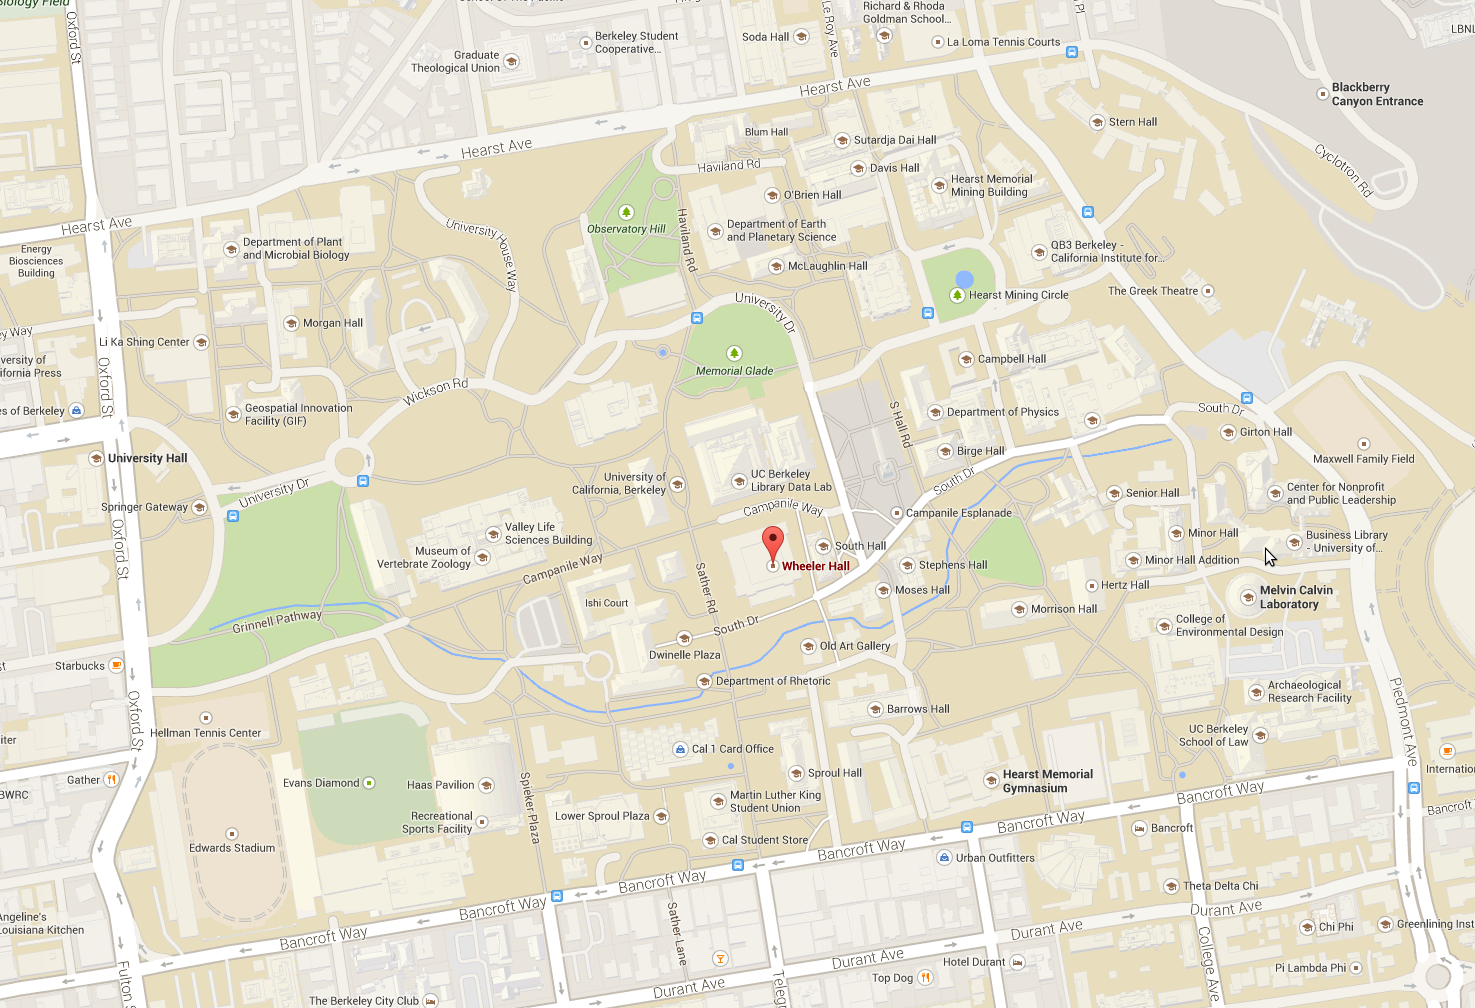
\includegraphics[width=\linewidth]{local_img/maps/wheeler_hall}
\end{figure}

The conference, workshops, and interactive poster sessions will take place in Wheeler Hall on the UC Berkeley campus. 

\newpage
\phantomsection \section{1st Floor -- Conference Venue}
{\large Monday, July 14 to Wednesday, July 16}
\begin{figure}[h!]
\center
\includegraphics[height=0.6\textheight]{local_img/maps/first_floor}
\end{figure}

\newpage
\phantomsection \section{Basement Floor -- Workshops Venue}
{\large Saturday, July 12 to Sunday, July 13}

\begin{figure}[h!]
\center
\includegraphics[height=0.6\textheight]{local_img/maps/basement}
\end{figure}

\newpage
\phantomsection \section{2nd Floor -- Workshops Venue}
{\large Saturday, July 12 to Sunday, July 13}

\begin{figure}[h!]
\center
\includegraphics[height=0.6\textheight]{local_img/maps/second_floor}
\end{figure}


\phantomsection \section{Banquet Information}
The conference banquet will be held on a cruise on the San Francisco Bay. Enjoy a splendid sunset on the water with magnificent views of the city of San Francisco, accompanied by a
delicious seasonal dinner and drinks. Transportation will be provided. Buses will pick us up from Berkeley at 6pm and take us to Pier 3 in San Francisco, where we will board the San Francisco Belle. Buses will pick us up from Pier 3 around 10pm, and we'll be back in Berkeley
around 10:30pm.

%\label{sec:banquetinfo}
%\begin{figure}[h!]
%\center
%\fbox{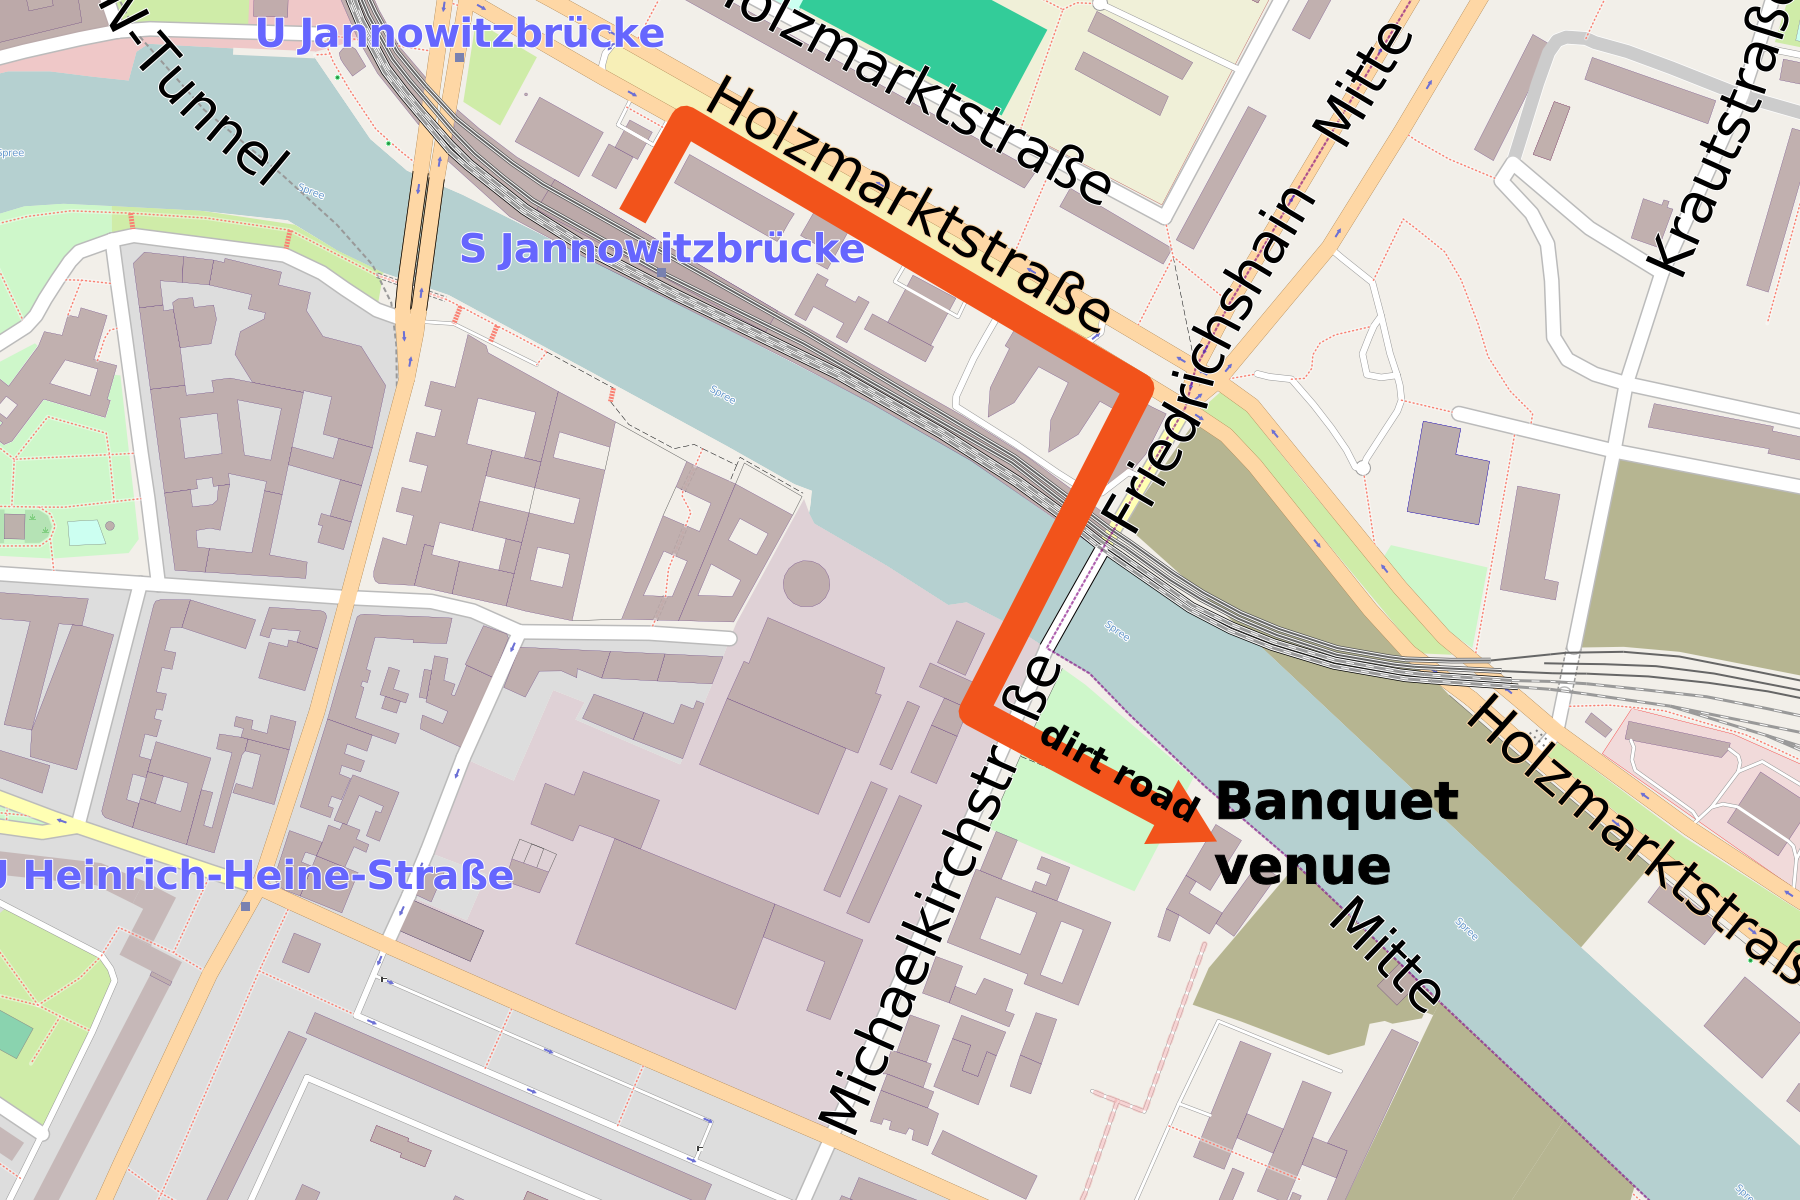
\includegraphics[width=3in]{local_img/maps/katerholzig_labeled}}
%\end{figure}

%After crossing the bridge, turn left through a boarded fence and enter the venue via an unpaved path. When you start wondering whether you are at the right place, you are at the right place.  Just keep on walking.  The address of Kater Holzig is Michaelkirchstra{\ss}e 23; the GPS coordinates are: 52.511283,13.42393. 

%The trip takes about 45 minutes. The banquet will begin at 20:00.


%\begin{landscape}
%\phantomsection \section{Public transport map}
%\begin{figure}[h!]
%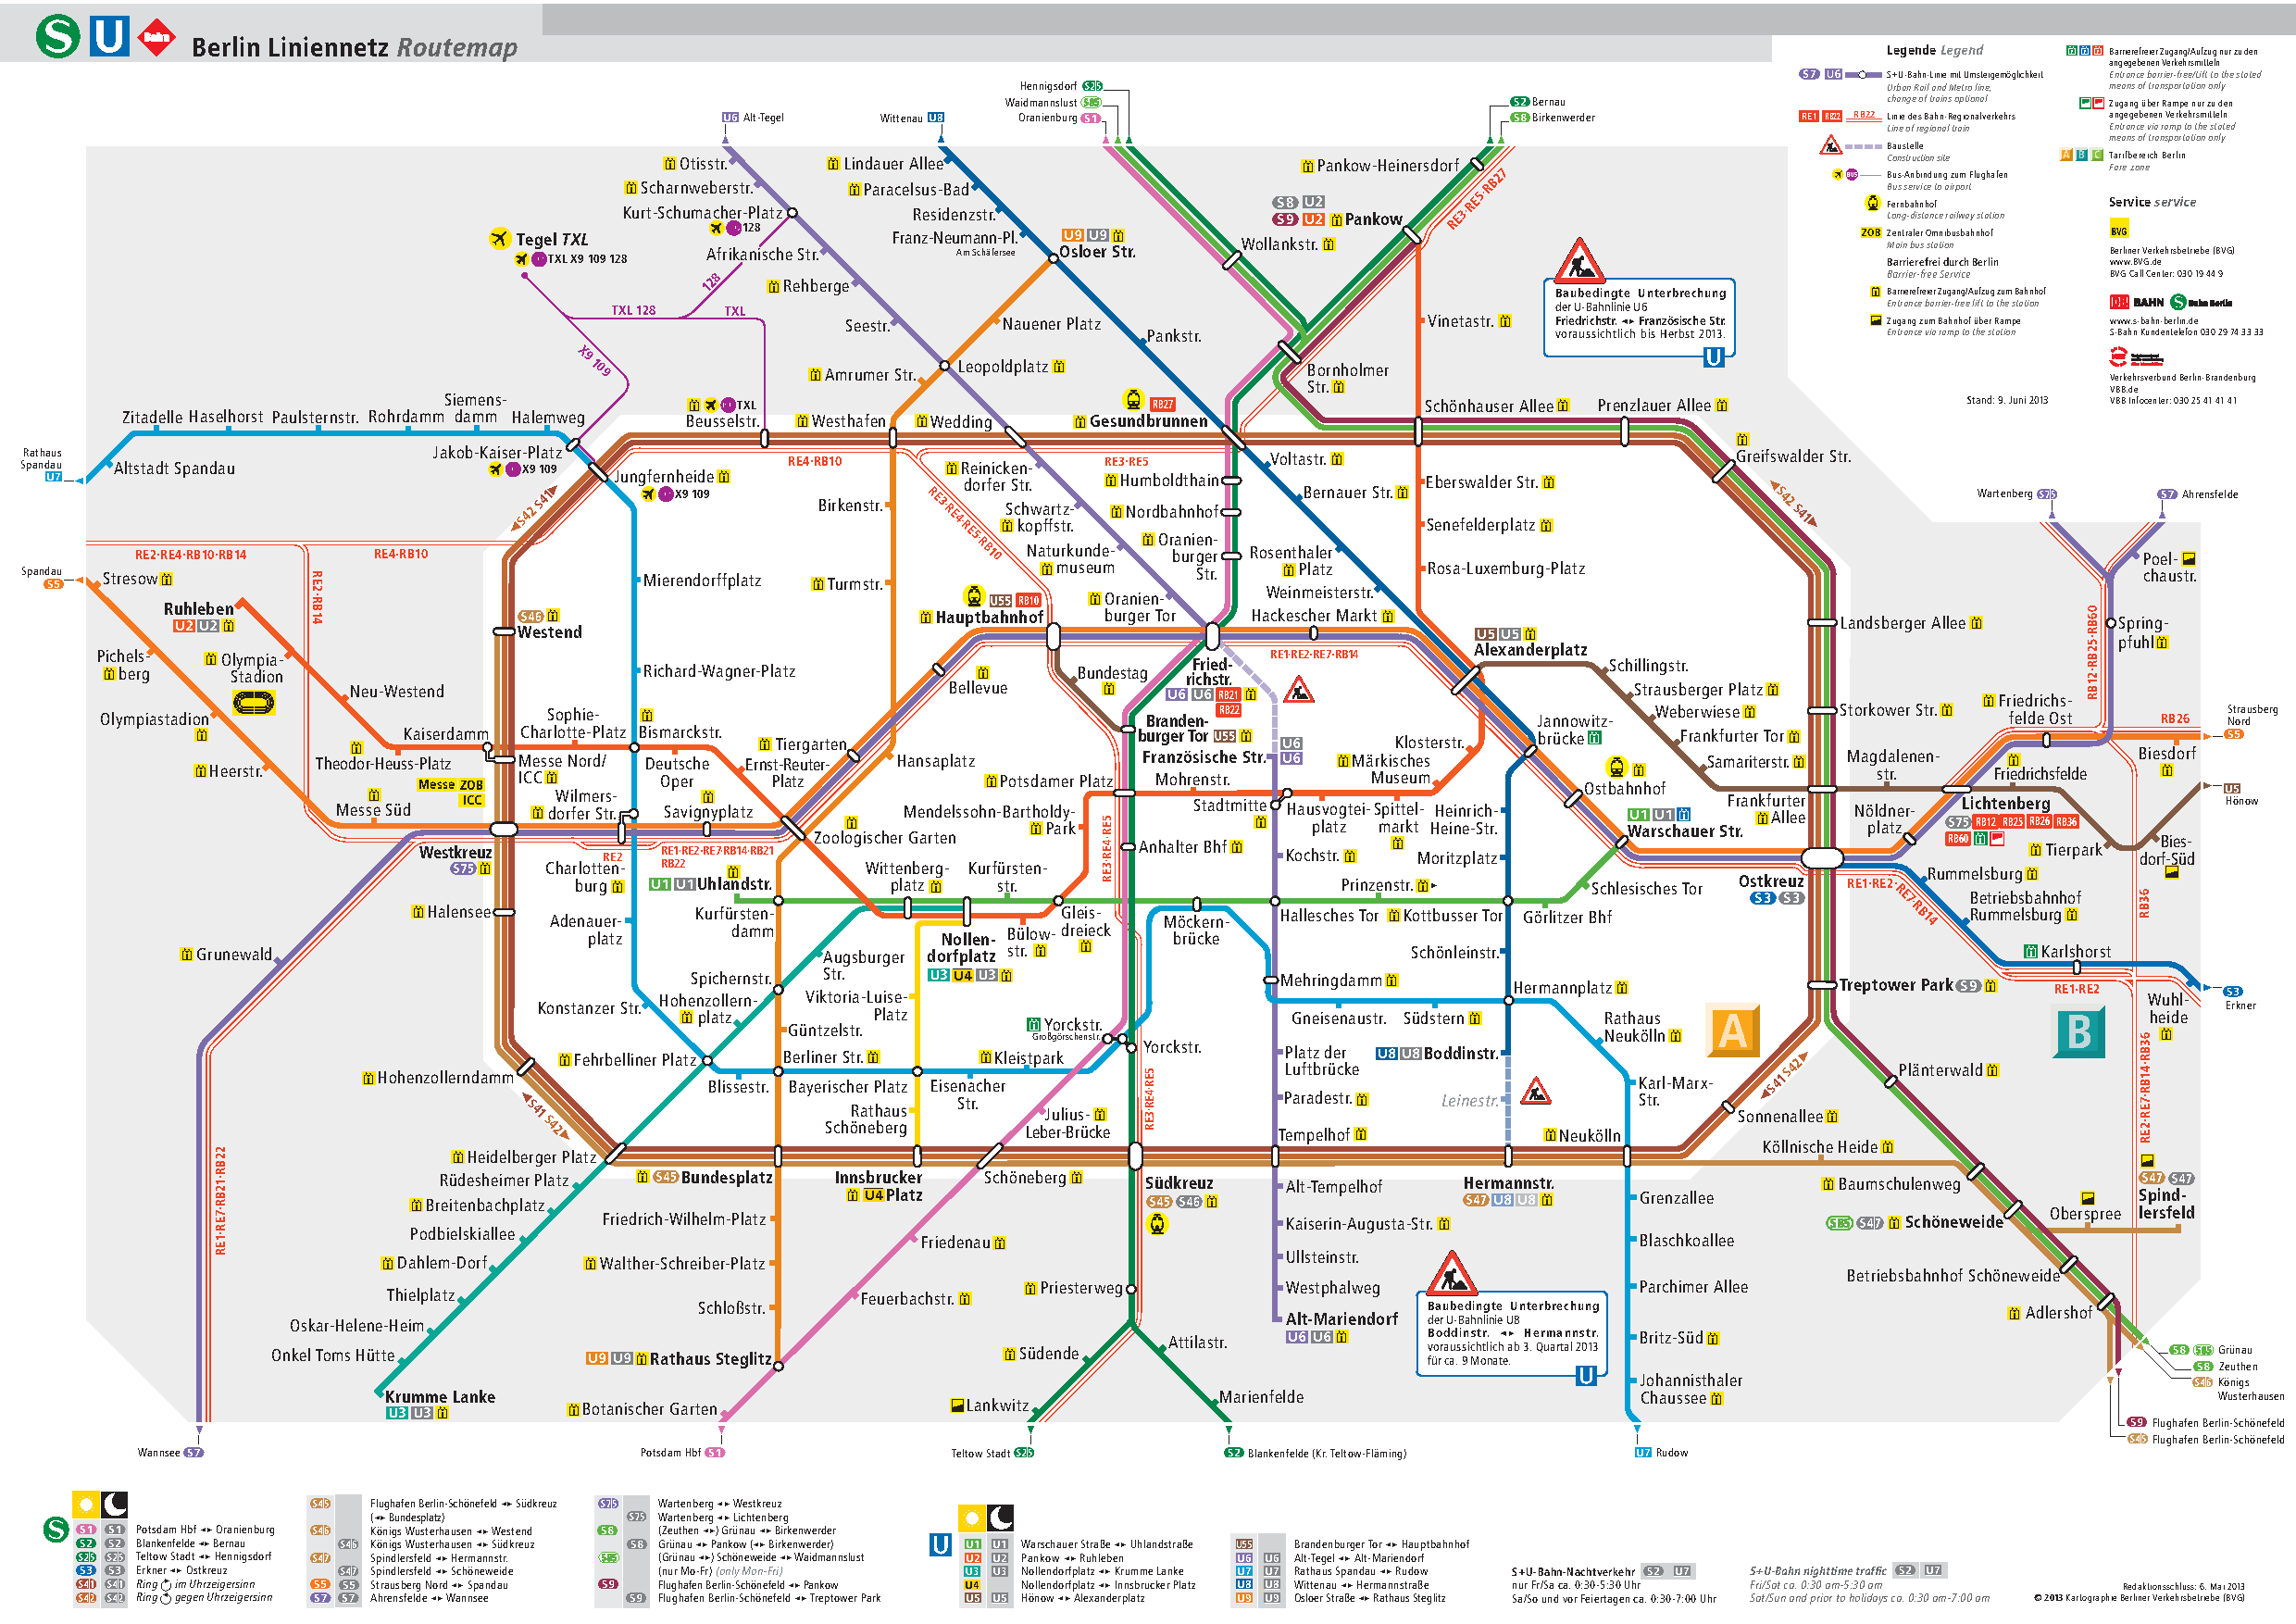
\includegraphics[height=0.9\textwidth, keepaspectratio]{local_img/maps/bvg}
%\end{figure}
%\end{landscape}


%set back fbox frame
\setlength\fboxrule{0pt}

    %contains sponsor information, about, general wuick info about arrangements

\chapter{Drink and Food Suggestions}

\setlength\fboxsep{0pt}
\setlength\fboxrule{0.5pt}

\vspace{-1.5cm}
\phantomsection \section{Lunch}

\begin{figure}[h!]
\center
\fbox{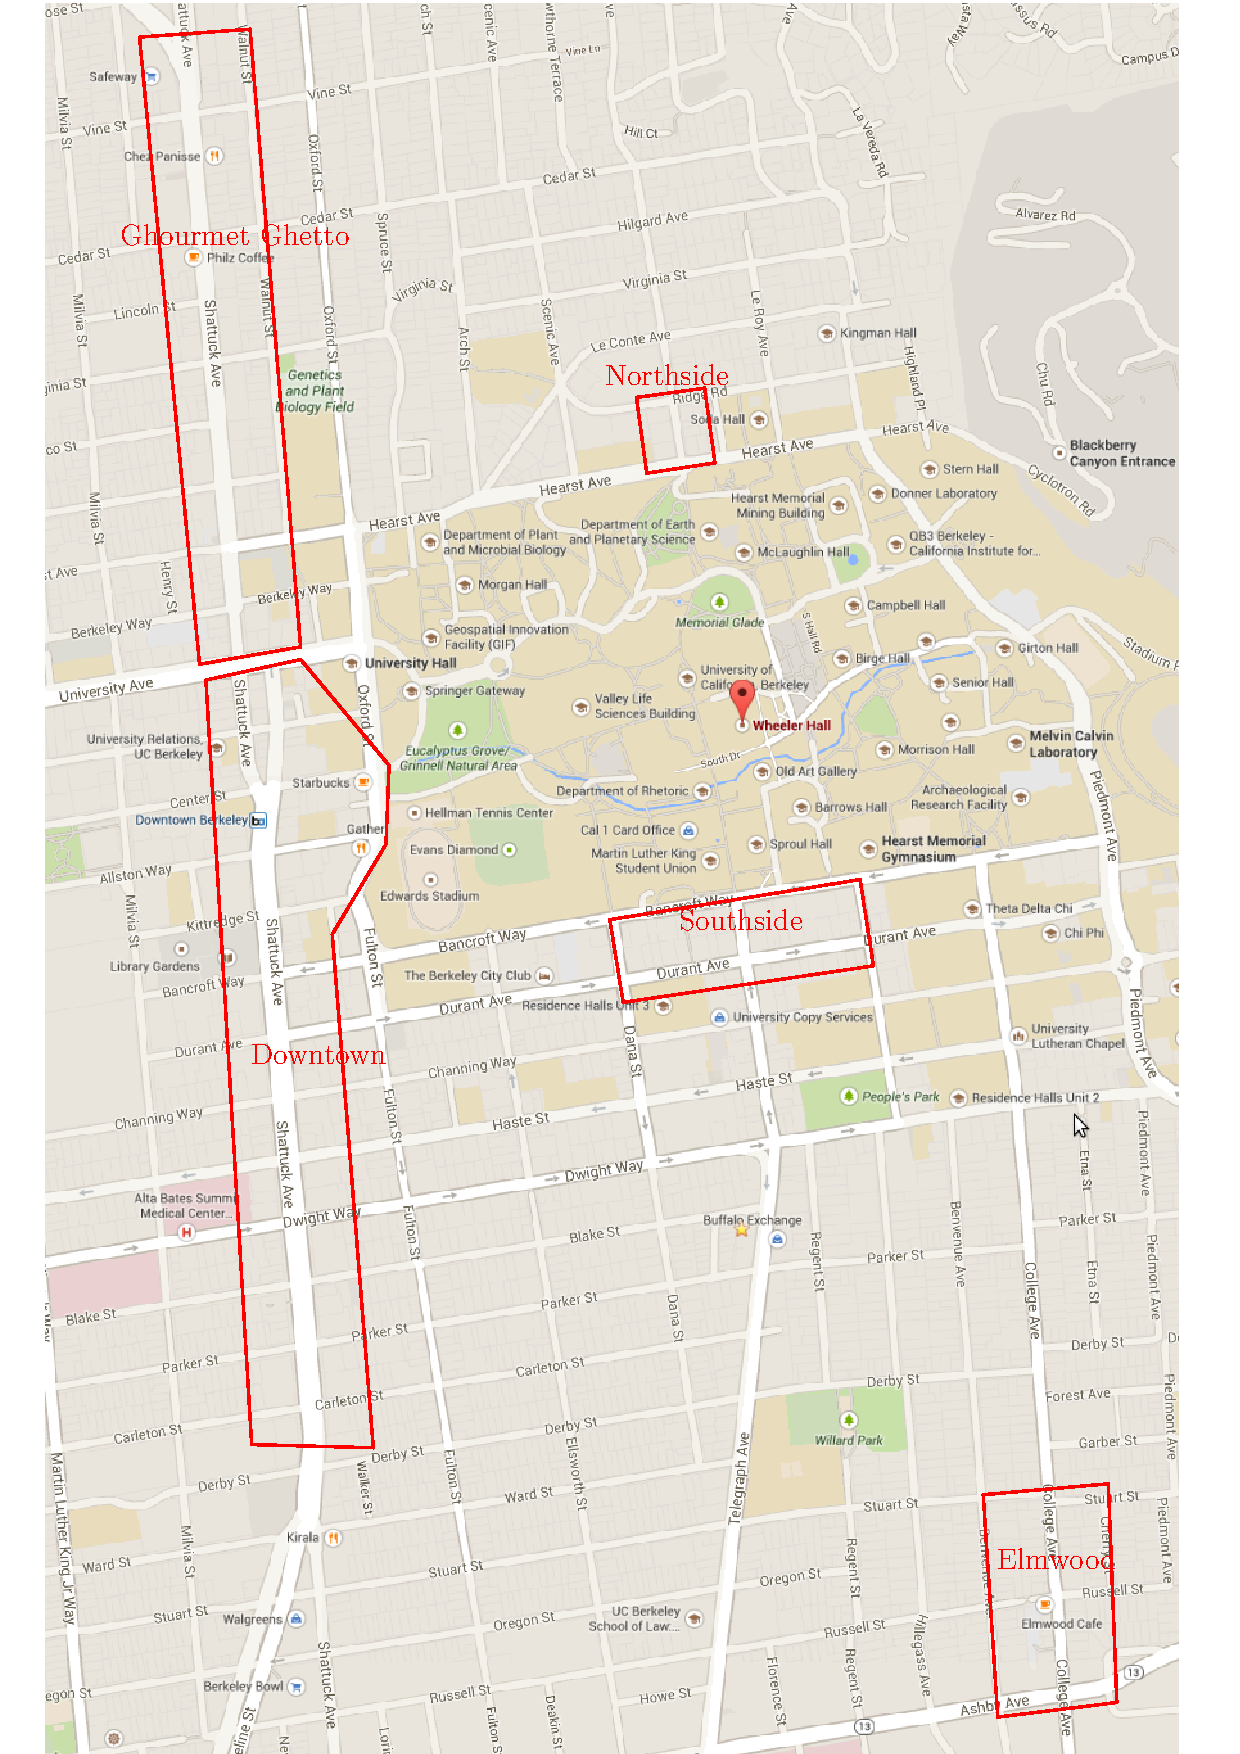
\includegraphics[width=6in]{local_img/maps/food.pdf}}
\end{figure}

We recommend the Southside, Northside, and Downtown neighborhoods for lunch in terms of proximity to the conference venue. We have provided below a sampling of lunch places in each of these neighborhoods, along with the type of food and price category. 

\vspace{1mm}

1) Southside (0.3 miles from Wheeler Hall)

\begingroup
\small
\begin{multicols}{1}[]
    \begin{tabular}{p{0.3cm} p{4cm} p{5cm} p{0.5cm}}
        1 & Cheese 'N' Stuff & Sandwiches & \$\\
        2 & Montague's Gourmet Sandwiches & Sandwiches & \$\\
        3 & Tivoli Caffe & Pizza, Sandwiches & \$\\
        4 & Gypsy's Trattoria Italiano & Italian  & \$\\
        5 & Julie's Cafe & Sandwiches, Salads & \$\\ 
        6 & KoJa Kitchen & Asian Fusion, Japanese & \$\\
        7 & Crepes A-Go Go & Creperie & \$\\
        8 & Chipotle Mexican Grill & Mexican & \$\\
        9 & Free House & Burgers, Salads, Sandwiches & \$\$\\
        10 & Henry's & Burgers, Salads, Sandwiches & \$\$\\
    \end{tabular}
\end{multicols}
\endgroup
\normalsize 

2) Northside (0.5 miles from Wheeler Hall)

\begingroup
\small
\begin{multicols}{1}[]
    \begin{tabular}{p{0.3cm} p{4cm} p{5cm} p{0.5cm}}
        1 & Northside Cafe & Breakfast, Sandwiches & \$\\
        2 & Urbann Turbann & Rice/Naan Wraps with Indian Curries & \$\\
        3 & D'Yar & Mediterranean & \$\\
        4 & The Pho Bar & Vietnamese  & \$\$\\
        5 & Cafe Nefeli & Mediterranean & \$\\ 
        6 & Bongo Burger & Burgers, Salads & \$\\
        7 & Celia's Mexican & Mexican & \$\$\\
        8 & Stuffed Inn & Sandwiches & \$\\
        9 & Jasmine Thai & Thai & \$\$\\
        10 & Hummingbird Cafe & Sandwiches, Mediterranean & \$\\
    \end{tabular}
\end{multicols}
\endgroup
\normalsize 

3) Downtown (1 mile from Wheeler Hall)

\begingroup
\small
\begin{multicols}{1}[]
    \begin{tabular}{p{0.3cm} p{4cm} p{5cm} p{0.5cm}}
        1 & Slow & Sandwiches & \$\\
        2 & Platano & Latin American & \$\$\\
        3 & Brazil Cafe & Brazilian, Sandwiches & \$\\
        4 & PIQ Bakery & Italian, Bakery  & \$\\
        5 & Sandwich Spot & Sandwiches & \$\\ 
        6 & Gecko Gecko & Thai & \$\$\\
        7 & Athineon & Mediterranean & \$\$\\
        8 & Sliver & Pizza, Sandwiches & \$\\
        9 & Toss Noodle Bar & Asian Fusion & \$\\
        10 & Suya African Caribbean Grill & African, Caribbean & \$\\
    \end{tabular}
\end{multicols}
\endgroup
\normalsize 

\phantomsection \section{Dinner}

There are a plethora of dining options available in the Berkeley neighborhoods listed on the map. We have provided below a sampling of dinner places that we like. This list is by no means comprehensive and we encourage you to check out dining options on Yelp! or Google maps as well. We recommend that you reserve a table in advance, especially on Saturday and Sunday.

\begingroup
\small
\begin{multicols}{1}[]
    \begin{tabular}{p{0.3cm} p{4cm} p{5cm} p{1cm} p{2cm}}
        1 & Gather & American, Drinks & \$\$ & Downtown \\
        2 & Jupiter & America, Drinks, Brewery & \$\$ & Downtown \\
	    3 & Comal & Mexican, Drinks & \$\$ & Downtown \\       
	    4 & Five & American, Drinks & \$\$\$ & Downtown \\ 
        5 & Cesar & Tapas Bar & \$\$\$ & Gourmet Ghetto\\
        6 & Cheese Board & Pizza & \$ & Gourmet Ghetto \\
        7 & Cha-Am & Thai & \$\$ & Gourmet Ghetto\\
        8 & Chez Panisse & French & \$\$\$\$ & Gourmet Ghetto \\
        9 & Taste of the Himalayas & Indian, Nepalese & \$\$ & Gourmet Ghetto \\
        10 & Henry's & American, Drinks & \$\$ & Southside \\
        11 & Free House & American, Drinks & \$\$ & Southside \\
        12 & Kiraku & Japanese Tapas & \$\$ & Southside \\
        13 & Wood Tavern & American, Drinks & \$\$\$ & Elmwood \\
        14 & Rangoon Super Stars & Burmese & \$\$ & Elmwood\\
        15 & Ici & Ice-cream & \$ & Elmwood\\
    \end{tabular}
\end{multicols}
\endgroup
\normalsize 

\setlength\fboxrule{0pt}
    %contains maps, event lists, and lunch/dinner/bar guides

\begingroup
%%%%%%%%%%%%%%%%%%%%%%%%%%%%%%%%%%%%%%%%%%%%%%%%%%%%
\chapter{Technical Program}
%%%%%%%%%%%%%%%%%%%%%%%%%%%%%%%%%%%%%%%%%%%%%%%%%%%%
\vspace{-15mm}
\phantomsection \section{General Schedule}


% Define event types
\defineevent{invited_talk}  {0.21}{0.5} {0.16}{1.0}{1.0}{1.0}
\defineevent{oralsession}   {0.0} {0.28}{1.0} {1.0}{1.0}{1.0}
\defineevent{workshop}      {0.8} {0.3} {0.15} {1.0}{1.0}{1.0}
\defineevent{poster_presentation} {1.0} {0.4} {0.2} {1.0}{1.0}{1.0}
\defineevent{event}   {0.75} {0.75} {1.0} {0.0}{0.0}{0.0}
\defineevent{break}   {1.0} {1.0} {1.0} {0.0}{0.0}{0.0}


%TODO: Add place of the coffee breaks!
\newcommand{\WorkshopsSchedule}[2]{
  \event #1 {0900} {1030} {09:00\\\vspace{0.2em}Workshops #2}        {90~min}                {Wheeler Hall}                   {workshop}
  \event #1 {1030} {1100} {10:30 Break}                              {\vspace{1.5mm}30 min}  {Wheeler Hall}     {break}
  \event #1 {1100} {1230} {11:00\\\vspace{0.2em}Workshops #2}        {90~min}                {Wheeler Hall}                   {workshop}
  \event #1 {1400} {1530} {14:00\\\vspace{0.2em}Workshops #2}        {90~min}                {Wheeler Hall}                   {workshop}
  \event #1 {1530} {1600} {15:30 Break}                              {\vspace{1.5mm}30 min}  {Wheeler Hall}     {break}
  \event #1 {1600} {1730} {16:00\\\vspace{0.2em}Workshops #2}        {90~min}                {Wheeler Hall}                   {workshop}
}

% Define the layout of your time tables
\setslotsize{3cm}{1.3mm}
\setslotcount {5} {168}
\settopheight{5}
\settextframe{1.5mm}
\setbottomspace{0pt}
% Start the time table
\begin{timetable}
  %define times to show:
  \hours{8}{5}{0}
  \englishdays{6}

  %thursday, workshop day 1
  \WorkshopsSchedule{1}{1-14}
  \event 1 {1230} {1400} {12:30\\\vspace{0.2em}Lunch Break}         {90~min}                {}                   {break}
  %friday, workshop day 2
  \WorkshopsSchedule{2}{14-24}
  \event 2 {1230} {1400} {12:30\\\vspace{0.2em}Lunch Break}         {90~min}                {}                   {break}

  %monday
  \event 3 {0830} {0900} {08:45 Welcome}                      {\vspace{1.5mm}15~min}          {\vspace{1.5mm}Room 150}        {event}
  \event 3 {0900} {1000} {09:00 Chris Urmson}                 {60~min}                        {Room 150}                      {invited_talk}
  \event 3 {1000} {1035} {10:00 Short Talks}                  {\vspace{1.5mm}35~min}          {\vspace{1.5mm}Room 150}        {oralsession}
  \event 3 {1035} {1130} {10:35 Break}                        {\vspace{1.5mm}55~min}          {Wheeler Hall}      {break}
  \event 3 {1130} {1235} {11:30 Talks}                        {\vspace{-0.5em}1~long + 6~short\\65~min}{Room 150}             {oralsession}
  \event 3 {1235} {1400} {12:35 Lunch Break}                  {85~min}                        {}                            {break}
  \event 3 {1400} {1500} {14:00 Genevieve Bell}               {60~min}                        {Room 150}                      {invited_talk}
  \event 3 {1500} {1530} {15:00 Short Talks} 		      {\vspace{1.5mm}30~min}          {\vspace{1.5mm}Room 150}        {oralsession}
  \event 3 {1530} {1645} {15:30 Break and Posters}            {\vspace{1.5mm}75~min}          {Wheeler Hall}      {break}
  \event 3 {1645} {1800} {16:45 Talks}                        {\vspace{-0.5em}1~long + 7~short\\75~min}{Room 150}             {oralsession}
  \event 3 {1800} {1930} {18:00 Reception}  	              {\vspace{1.5mm}90~min}          {Wheeler Hall}        {event}


  %tuesday
  \event 4 {0900} {1000} {09:00 Brad Nelson}                 {60~min}                        {Room 150}                      {invited_talk}
  \event 4 {1000} {1035} {10:00 Short Talks}                  {\vspace{1.5mm}35~min}          {\vspace{1.5mm}Room 150}        {oralsession}
  \event 4 {1035} {1130} {10:35 Break and Posters}            {\vspace{1.5mm}55~min}          {Wheeler Hall}      {break}
  \event 4 {1130} {1235} {11:30 Talks}                        {\vspace{-0.5em}1 long + 6 short\\65~min}{Room 150}             {oralsession}
  \event 4 {1235} {1400} {12:35\\[0.2em]Lunch Break}          {85~min}                        {}                            {break}
  \event 4 {1400} {1530} {14:00 Talks}                        {\vspace{-0.5em}2 long + 6 short\\90~min}{Room 150}             {oralsession}
  \event 4 {1530} {1645} {15:30 Break and Posters}            {\vspace{1.5mm}75~min}          {Wheeler Hall}      {break}
  \event 4 {1645} {1800} {16:45 Talks}                        {\vspace{-0.5em}1 long + 6 short\\75~min}{Room 150}             {oralsession}
  \event 4 {1800} {2000} {18:00\\\vspace{0.3em}Buses Depart for Banquet}       {2~h}          {\vspace{-0.7em}at San Francisco Bay}     {event}



  %wednesday
  \event 5 {0900} {1000} {09:00 Andrew Ng}                            {60~min}                           {Room 150}                      {invited_talk}
  \event 5 {1000} {1042} {10:00 Short Talks}                          {\vspace{1.5mm}42~min}             {\vspace{1.5mm}Room 150}        {oralsession}
  \event 5 {1042} {1140} {10:30 Break and Posters}                    {\vspace{1.5mm}58 min}             {Wheeler Hall}      {break}
  \event 5 {1140} {1210} {11:40 Forum}                                {\vspace{1.5mm}30~min}             {\vspace{1.5mm}Room 150}                      {event}
  \event 5 {1210} {1400} {12:10\\[0.2em]Lunch and Lab Tours}          {110~min}                          {}                            {break}
  \event 5 {1400} {1500} {14:00 Nancy Amato}                          {60~min}                           {Room 150}                      {invited_talk}
  \event 5 {1500} {1600} {15:00 Early Career Spotlights} 	      {\vspace{1.5mm}60~min}             {\vspace{1.5mm}Room 150}        {event}
  \event 5 {1600} {1630} {16:00 Awards} 	              {\vspace{1.5mm}15~min}             {\vspace{1.5mm}Room 150}        {event}
  \event 5 {1630} {1705} {16:15 Farewell} 	              {\vspace{1.5mm}45~min}             {Wheeler Hall}        {break}
  \event 5 {1705} {2000} {17:00\\\vspace{0.3em}Evening at Google}     {3~h}                              {at Google}     {event}
\end{timetable}






%%%%%%%%%%general config for the tables:
\begingroup %limit the changes to the schedule tables
\sffamily


%how to format each talk:
\ifthenelse{\equal{\targetoutput}{print}}{      \newcommand{\addpaper}[5]{ #3: #1                        & #2     & #4 }  }{}
\ifthenelse{\equal{\targetoutput}{usbstick}}{   
   \newcommand{\addpaper}[5]{ 
       \href{proceedings/#3.pdf}{#1}
       \ifthenelse{\equal{#5}{}}{}{
          (\href{proceedings/supplementary/#5}{supplementary})
       }
       & #2     
       & #4
   }  
}{}

\ifthenelse{\equal{\targetoutput}{online}}{   
   \newcommand{\addpaper}[5]{ 
       \href{http://roboticsproceedings.org/rss10/#3.pdf}{#1}
       & #2     
       & #4
   }  
}{}


\newcommand{\addtalk}[2]{ #1 & #2 &}
\newcommand{\timeemph}[1]{\hline \\[-4mm] {\Large#1}}
\newcommand{\begindailyscheduletabular}{ %config of the schedule tabular
    \begin{tabular}{>{\small}r>{\footnotesize}r>{\small}p{14.5cm}>{\footnotesize \raggedright}p{6cm}>{\small}r}
    {\footnotesize Start}&{\footnotesize Length}& & \multicolumn{2}{r}{\footnotesize Interactive session ID}\\
}
%%%%%%%%%%%%%%%%%%%%%%%%%%%%%%%%%%%%%%
\clearpage
\begin{landscape}

%how to format each talk:
\ifthenelse{\equal{\targetoutput}{print}}{      \newcommand{\addworkshop}[5]{#3 &           #1  & #2 & #4 \\ \hline} }{}
\ifthenelse{\equal{\targetoutput}{usbstick}}{   \newcommand{\addworkshop}[5]{#3 & \href{#5}{#1} & #2 & #4 \\ \hline} }{}
\ifthenelse{\equal{\targetoutput}{online}}{     \newcommand{\addworkshop}[5]{#3 & \href{#5}{#1} & #2 & #4 \\ \hline} }{}


\renewcommand{\arraystretch}{2.0}
\setlength{\tabcolsep}{7pt}
\clearpage
\phantomsection \section{Saturday, July 12: Workshops SAT1-SAT14}
\begin{tabular}{>{\small}rr>{\raggedright}p{14cm}>{\small \raggedright}p{3.5cm}>{\small}r}
\normalsize ID & \normalsize Room & \normalsize Title & \normalsize Chair & \normalsize Notes\\
\hline
SAT1 & \addworkshop{5th Workshop on Formal Methods for Robotics and Automation}{H. Kress-Gazit, C. Belta}{4.063}{}{http://verifiablerobotics.com/RSS14/index.html}
SAT2 & \addworkshop{5th Workshop on RGB-D Perception: Reconstruction and Recognition}{H. Koppula, J. Xiao, A. Saxena, J. Leonard}{0.003}{}{http://www.cs.cornell.edu/~hema/rgbd-workshop-2014/}
SAT3 & \addworkshop{Autonomous Control, Adaptation, and Learning for Underwater Vehicles}{G. Hollinger, M. Hsieh, F. Hover, R. Smith}{0.010}{}{http://drexelsaslab.appspot.com/workshops/rss2014/index.html}
SAT4 & \addworkshop{DARPA Robotics Challenge: Lessons Learned and What's Next}{M. Fallon and S. Kuindersma}{0.015}{}{http://drcworkshop.csail.mit.edu/}
SAT5 & \addworkshop{Distributed Control and Estimation for Robotic Vehicle Networks}{N. Ahmed, S. Martinez, J. Cortes}{0.016}{}{https://sites.google.com/site/rss2014dceworkshop}
SAT6 & \addworkshop{Human versus Robot Grasping and Manipulation—How Can We Close the Gap?}{O. Brock, D. Berenson, J. Mainprice, M. Roa, C. Eppner}{0.007}{}{http://www.mobilemanipulation.org/rss2014}
SAT7 & \addworkshop{Human–Robot Collaboration for Industrial Manufacturing}{A. Sauppe, M. Gombolay, J. Shah, B. Mutlu}{0.002}{}{http://hci.cs.wisc.edu/workshops/RSS2014/}
SAT8 & \addworkshop{Moral, Ethical, and Legal Issues in Robotics}{J. Gillula, J. Urban}{0.001}{}{http://hybrid.eecs.berkeley.edu/workshops/2014/RSS/law-ethics/}
SAT9 & \addworkshop{Non-parametric Learning in Robotics}{R. Triebel, L. Spinello}{0.011}{}{http://ais.informatik.uni-freiburg.de/nonparam_rss14/index.html}
SAT10 & \addworkshop{Optimization techniques for motion generation in robotics}{A. Escande, K. Mombaur}{0.017}{}{http://www.orb.uni-hd.de/conferences-workshops/RSS2014}
SAT11 & \addworkshop{Resource-efficient Integration of Planning and Perception for true autonomous operation of Micro Air Vehicles (MAVs)}{D. Burschka, M. Suppa, R. Siegwart, K. Schmid, M. Achtelik}{0.008}{}{http://rss2014_uav.visual-navigation.com/}
SAT12 & \addworkshop{Robot makers: The future of digital rapid design and fabrication of robots}{A. Mehta, M. Tolley, N. Bezzo, C. Onal}{4.065}{}{http://www.seas.upenn.edu/~nicbezzo/RoMa2014/}
SAT13 & \addworkshop{Workshop on Robotics Methods for Structural and Dynamic Modeling of Molecular Systems}{L. Tapia, J. Corts, J. J. Cheng, A. Shehu, K. Manavi}{0.009}{}{https://cs.unm.edu/amprg/rss14workshop/}
SAT14 & \addworkshop{Workshop on Women in Robotics}{J. Pineau, A. Tomaz, M. Bennewitz, L. Takayama}{4.064}{}{http://www.cs.mcgill.ca/~jpineau/rss14-wir.html}


\end{tabular}
\vfill


\clearpage
\phantomsection \section{Sunday, July 13: Workshops SUN1-SUN14}
\begin{tabular}{>{\small}rr>{\raggedright}p{14cm}>{\small \raggedright}p{3.5cm}>{\small}r}
\normalsize ID & \normalsize Room & \normalsize Title & \normalsize Chair & \normalsize Notes\\
\hline
SUN1 & \addworkshop{Affordances in Vision for Cognitive Robotics}{K. M. Varadarajan, M. Vincze, T. Darrell, J. Gall}{4.064}{}{http://affordances.info/workshops/RSS.html}
SUN2 & \addworkshop{Communication-aware Robotics: New Tools for Multi-Robot Networks, Autonomous Vehicles, and Localization}{D. Rus, S. Gil, N. Ayanian, S. Kumar}{4.063}{}{http://groups.csail.mit.edu/drl/wiki/index.php?title=RSS_2014_Proposed_Workshop}
SUN3 & \addworkshop{Constrained decision-making in robotics: models, algorithms, and applications}{S Carpin, M. Pavone}{0.001}{}{http://robotics.ucmerced.edu/RSS2014Workshop}
SUN4 & \addworkshop{Dynamic Locomotion}{A. Ames, K. Sreenath}{0.002}{}{http://www.dynamiclocomotion.org/}
SUN5 & \addworkshop{Guaranteed Safety for Uncertain Robotic Systems}{J. Gillula, S. Kaynama}{0.007}{}{http://hybrid.eecs.berkeley.edu/workshops/2014/RSS/safety}
SUN6 & \addworkshop{Humans and Sensing in Cyber-Physical Systems}{A. Aswani, R. Vasudevan}{0.008}{}{http://ieor.berkeley.edu/~aaswani/rss14_cps/}
SUN7 & \addworkshop{Information-based Grasp and Manipulation Planning}{S. Patil, R. Platt Jr.}{0.010}{}{http://rll.berkeley.edu/RSS2014Workshop}
SUN8 & \addworkshop{Learning plans with context from Human signals}{D Bagnell, A. Jain, J. Peters, A. Saxena}{0.011}{}{http://learningplans.cs.cornell.edu/}
SUN9 & \addworkshop{Managing Software Variability in Robot Control Systems}{D. Brugali, C. Schlegel}{0.016}{Half day}{http://robotics.unibg.it/tcsoft/rss2014/}
SUN10 & \addworkshop{Next-Generation Robotics: Academia, Start-ups and Industry}{S. Chitta, I. Sucan, T. Kroeger}{0.017}{}{http://moveit.ros.org/rss-2014-workshop/}
SUN11 & \addworkshop{Self-Driving Vehicles: Technology and Policy}{J. Leonard, J. Levinson}{4.065}{}{http://jleonard.scripts.mit.edu/sdv/}
SUN12 & \addworkshop{Advances on Soft Robotics}{C. Laschi, F. Iida, J. Rossiter, L. Margheri}{4.065}{}{http://www.robosoftca.eu/events/RSS2014-workshop/}
SUN13 & \addworkshop{Workshop on Multi-View Geometry in Robotics (MVIGRO 2014)}{V. Indelman, L. Carlone, F. Dellaert}{4.065}{}{http://www.cc.gatech.edu/events/mvigro/}
SUN14 & \addworkshop{Workshop on Robotic Monitoring}{A. Breitenmoser, J. Muller, J. Das, R. Smith, C. Detweiler}{4.065}{}{http://cinaps.usc.edu/rss2014/}

\end{tabular}
\vfill


\renewcommand{\arraystretch}{1.8}
\setlength{\tabcolsep}{7pt}

\clearpage
\phantomsection \section{Monday Morning, July 14}
\begindailyscheduletabular
\timeemph{08:45} & 15 & Welcome &&\\
\timeemph{09:00} & 60 & \addtalk{Invited Talk: Realizing Self-Driving Cars}{Chris~Urmson}\\
10:00&7& \addpaper{Batch Continuous-Time Trajectory Estimation as Exactly Sparse Gaussian Process Regression}{Tim~Barfoot, Chi~Hay~Tong, Simo~Sarkka}{p01}{A1}{}\\
&7& \addpaper{Combining 3D Shape, Color, and Motion for Robust Anytime Tracking}{David~Held, Jesse~Levinson, Sebastian~Thrun, Silvio~Savarese}{p14}{A2}{}\\
&7& \addpaper{Decision-Making Authority, Team Efficiency and Human Worker Satisfaction in Mixed Human-Robot Teams}{Matthew~Gombolay, Reymundo~Gutierrez, Giancarlo~Sturla, Julie~Shah}{p46}{A3}{}\\
&7& \addpaper{Stiction Compensation in Agonist-Antagonist Variable Stiffness Actuators}{Luca~Fiorio, Francesco~Romano, Alberto~Parmiggiani, Giulio~Sandini, Francesco~Nori}{p32}{A4}{}\\
&7& \addpaper{Simultaneous Compliance and Registration Estimation for Robotic Surgery}{Siddharth~Sanan, Stephen~Tully, Andrea~Bajo, Nabil~Simaan, Howie~Choset}{p51}{A5}{}\\
\timeemph{10:35} &55 &Coffee Break & &\\
\timeemph{11:30}&25&\addpaper{Vision-based Landing Site Evaluation and Trajectory Generation Toward Rooftop Landing}{Vishnu~Desaraju, Nathan~Michael, Martin~Humenberger, Roland~Brockers, Stephan~Weiss, Larry~Matthies}{p44}{B1}{}\\
11:55&7& \addpaper{Correct High-level Robot Behavior in Environments with Unexpected Events}{Kai~Weng~Wong, Rudiger~Ehlers, Hadas~Kress-Gazit}{p12}{B2}{}\\
&7& \addpaper{Persistent Monitoring of Stochastic Spatio-temporal Phenomena with a Small Team of Robots}{Sahil~Garg, Nora~Ayanian}{p38}{B3}{}\\
&7& \addpaper{Modeling and Controlling Friendliness for An Interactive Museum Robot}{Chien-Ming~Huang, Takamasa~Iio, Satoru~Satake, Takayuki~Kanda}{p25}{B4}{}\\
&7& \addpaper{Efficient Visual-Inertial Navigation using a Rolling-Shutter Camera with Inaccurate Timestamps}{Chao~Guo, Dimitrios~Kottas, Ryan~DuToit, Ahmed~Ahmed, Ruipeng~Li, Stergios~Roumeliotis}{p57}{B5}{}\\
&7& \addpaper{Dynamically Feasible Motion Planning through Partial Differential Flatness}{Suresh~Ramasamy, Guofan~Wu, Koushil~Sreenath}{p53}{B6}{}\\
&7& \addpaper{Sky Segmentation with Ultraviolet Images Can Be Used for Navigation}{Thomas~Stone, Michael~Mangan, Paul~Ardin, Barbara~Webb}{p47}{B7}{}\\
\timeemph{12:35} &95& Lunch Break && \\
\hline
\end{tabular}
\vfill

\clearpage
\phantomsection \section{Monday Afternoon, July 14}
\begindailyscheduletabular
\timeemph{14:00} &60& \addtalk{Invited Talk: The Pre-history of Robots}{Genevieve Bell} \\
15:00&7& \addpaper{Hierarchical Semantic Labeling for Task-Relevant RGB-D Perception}{Chenxia~Wu, Ian~Lenz, Ashutosh~Saxena}{p06}{C1}{}\\
&7& \addpaper{Multi-Heuristics A*}{Sandip~Aine, Siddharth~Swaminathan, Venkatraman~Narayanan, Victor~Hwang, Maxim~Likhachev}{p56}{C2}{}\\
&7& \addpaper{Learning Articulated Motions from Visual Demonstration}{Sudeep~Pillai, Matthew~Walter, Seth~Teller}{p50}{C3}{}\\
&7& \addpaper{An Analysis of Deceptive Robot Motion}{Anca~Dragan, Rachel~Holladay, Siddhartha~Srinivasa}{p10}{C4}{}\\
\timeemph{15:30} &75& Coffee Break and Posters (A1-A5, B1-B7, C1-C4) && \\
16:45&25& \addpaper{Semantic Localization Via the Matrix Permanent}{Nikolay~Atanasov, Menglong~Zhu, Kostas~Daniilidis, George~Pappas}{p43}{D1}{}\\
17:10&7& \addpaper{The Multi-Agent Navigation Transformation: Tuning-Free Multi-Robot Navigation}{Savvas~Loizou}{p17}{D2}{}\\
&7& \addpaper{An Automata-Theoretic Approach to the Vehicle Routing Problem}{Cristian~Vasile, Calin~Belta}{p45}{D3}{}\\
&7& \addpaper{Effective Task Training Strategies for Instructional Robots}{Allison~Sauppe, Bilge~Mutlu}{p02}{D4}{}\\
&7& \addpaper{Learning to Locate from Demonstrated Searches}{Paul~Vernaza, Anthony~Stentz}{p35}{D5}{}\\
&7& \addpaper{Modeling High-Dimensional Humans for Activity Anticipation using Gaussian Process Latent CRFs}{Yun~Jiang, Ashutosh~Saxena}{p15}{D6}{}\\
&7& \addpaper{Manhattan and Piecewise-Planar Constraints for Dense Monocular Mapping}{Alejo~Concha, Wajahat~Hussain, Luis~Montano, Javier~Civera}{p16}{D7}{}\\
&7& \addpaper{Appearance-based Active, Monocular, Dense Reconstruction for Micro Aerial Vehicles}{Christian~Forster, Matia~Pizzoli, Davide~Scaramuzza}{p29}{D8}{}\\
\timeemph{18:00}& 90& Reception & \\
\hline
\end{tabular}
\vfill

%%%%%%%%%%%%%%%%%%
\clearpage
\phantomsection \section{Tuesday Morning, July 15}
\begindailyscheduletabular
\timeemph{09:00}  & 60&\addtalk{Invited Talk: Swimming Microrobots}{Brad~Nelson}\\
10:00&7& \addpaper{Bio-Artificial Synergies for Grasp Posture Control of Supernumerary Robotic Fingers}{Faye~Wu, Harry~Asada}{p27}{E1}{}\\
&7& \addpaper{Six-Degrees-of-Freedom Remote Actuation of Magnetic Microrobots}{Eric~Diller, Joshua~Giltinan, Guo~Zhan~Lum, Zhou~Ye, Metin~Sitti}{p13}{E2}{}\\
&7& \addpaper{5-DOF Manipulation of an Untethered Magnetic Device in Fluid using a Single Permanent Magnet}{Arthur~Mahoney, Abbott~Jake}{p37}{E3}{}\\
&7& \addpaper{Automatic Generation of Reduced CPG Control Networks for Locomotion of Arbitrary Modular Robot Structures}{Stephane~Bonardi, Massimo~Vespignani, Rico~Moeckel, Jesse~Van~den~Kieboom, Soha~Pouya, Alexander~Sproewitz, Auke~Ijspeert}{p04}{E4}{}\\
&7& \addpaper{Cogging Torque Ripple Minimization via Position Based Characterization }{Matthew~Piccoli, Mark~Yim}{p42}{E5}{}\\

\timeemph{10:35} &55 &Coffee Break and Posters (D1-D8, E1-E5) && \\

\timeemph{11:30}&25& \addpaper{A Novel Type of Compliant, Underactuated Robotic Hand for Dexterous Grasping}{Raphael~Deimel, Oliver~Brock}{p18}{F1}{}\\
11:55&7& \addpaper{Pre- and Post-Contact Policy Decomposition for Planar Contact Manipulation Under Uncertainty}{Michael~Koval, Nancy~Pollard, Siddhartha~Srinivasa}{p34}{F2}{}\\
&7& \addpaper{Modeling Robot Discrete Movements with State-varying Stiffness and Damping: A framework for integrated motion generation and impedance control}{Mohammad~Khansari, Klas~Kronander, Aude~Billard}{p22}{F3}{}\\
&7&  \addpaper{Robust Policies via Meshing for Metastable Rough Terrain Walking}{Cenk~Oguz~Saglam, Katie~Byl}{p49}{F4}{}\\
&7&  \addpaper{Probably Approximately Correct MDP Learning and Control With Temporal Logic Constraints}{Jie~Fu, Ufuk~Topcu}{p39}{F5}{}\\
&7&  \addpaper{Self-Calibration and Visual SLAM with a Multi-Camera System on a Micro Aerial Vehicle}{Lionel~Heng, Gim~Hee~Lee, Marc~Pollefeys}{p08}{F6}{}\\
&7&  \addpaper{Control of Robotic Mobility-On-Demand Systems: a Queueing-Theoretical Perspective}{Rick~Zhang, Marco~Pavone}{p26}{F7}{}\\
\timeemph{12:35} &55& Lunch Break && \\
\hline
\end{tabular}
\vfill

\clearpage
\phantomsection \section{Tuesday Afternoon, July 15}
\begindailyscheduletabular
\timeemph{14:00} &25& \addpaper{Multiscale Topological Trajectory Classification with Persistent Homology}{Florian~Pokorny, Majd~Hawasly, Subramanian~Ramamoorthy}{p54}{G1}{}\\
14:25&25&  \addpaper{Asking for Help Using Inverse Semantics}{Stefanie~Tellex, Ross~Knepper, Adrian~Li, Daniela~Rus, Nicholas~Roy}{p24}{G2}{}\\
14:50&7&  \addpaper{LOAM: Lidar Odometry and Mapping in Real-time}{Ji~Zhang, Sanjiv~Singh}{p07}{G3}{}\\
&7&  \addpaper{Combining the Benefits of Function Approximation and Trajectory Optimization}{Igor~Mordatch, Emo~Todorov}{p52}{G4}{}\\
&7&  \addpaper{Enhanced 3D Kinematic Modeling of Wheeled Mobile Robots}{Neal~Seegmiller, Alonzo~Kelly}{p20}{G5}{}\\
&7&  \addpaper{Tell Me Dave: Context-Sensitive Grounding of Natural Language to Manipulation Instructions}{Dipendra~Kumar Misra, Jaeyong~Sung, Kevin~Lee, Ashutosh~Saxena}{p05}{G6}{}\\
&7&  \addpaper{Nonlinear Graph Sparsification for SLAM}{Mladen~Mazuran, Tipaldi~Gian~Diego, Spinello~Luciano, Wolfram~Burgard}{p40}{G7}{}\\
&7&  \addpaper{Fully Decentralized Task Swaps with Optimized Local Searching}{Lantao~Liu, Nathan~Michael, Dylan~Shell}{p21}{G8}{}\\
\timeemph{15:30} &75& Coffee Break and Posters (F1-F7, G1-G8) &&\\
\timeemph{16:45} &25& \addpaper{Robot Programming by Demonstration with Interactive Action Visualizations}{Sonya~Alexandrova, Maya~Cakmak, Kaijen~Hsiao, Leila~Takayama}{p48}{H1}{}\\
17:10&7&  \addpaper{An Online Sparsity-Cognizant Loop-Closure Algorithm for Visual Navigation}{Yasir~Latif, Guoquan~Huang, John~Leonard, Jose~Neira}{p36}{H2}{}\\
&7&  \addpaper{Scene Signatures: Localised and Point-less Features for Localisation}{Colin~McManus, Ben~Upcroft, Paul~Newmann}{p23}{H3}{}\\
&7&  \addpaper{Active Reward Learning}{Christian~Daniel, Malte~Viering, Jan~Metz, Oliver~Kroemer, Jan~Peters}{p31}{H4}{}\\
&7&  \addpaper{Learning to Recognize Human Activities from Soft Labeled Data}{Ninghang~Hu, Zhongyu~Lou, Gwenn~Englebienne, Ben~Krose}{p03}{H5}{}\\
&7&  \addpaper{Planning Single-arm Manipulations with n-Arm Robots}{Benjamin~Cohen, Mike~Phillips, Maxim~Likhachev}{p33}{H6}{}\\
&7&  \addpaper{Robust and Agile 3D Biped Walking with Steering Capability Using a Footstep Predictive Approach}{Salman~Faraji, Soha~Pouya, Auke~Ijspeert}{p28}{H7}{}\\
\timeemph{18:00}& & Buses Depart for Banquet & \\
\hline
\end{tabular}
\vfill

%%%%%%%%%%%%%%%%%%%%%%%%%%%%%%%%%%%%%%
\clearpage
\phantomsection \section{Wednesday, July 16}
\begindailyscheduletabular
\timeemph{09:00}  & 60&\addtalk{Invited Talk: Deep Learning: Machine Learning via Large-scale Brain Simulations}{Andrew~Ng}\\
10:00&7& \addpaper{Open-vocabulary Object Retrieval}{Sergio~Guadarrama, et~al.}{p41}{I1}{}\\
&7& \addpaper{State Representation Learning in Robotics: Using Prior Knowledge about Physical Interaction}{Rico~Jonschkowski, Oliver~Brock}{p19}{I2}{}\\
&7& \addpaper{Conditioned Basis Array Factorization: An Approach to Gait Pattern Extraction}{Chaohui~Gong, Matthew~Travers, Henry~Astley, Lu~Li, Joseph~Mendelson, David~Hu, Daniel~Goldman, Howie~Choset}{p55}{I3}{}\\ 
&7& \addpaper{Online Trajectory Planning in Dynamic Environment for Surgical Task Automation}{Takayuki~Osa, Naohiko~Sugita, Mamoru~Mitsuishi}{p11}{I4}{}\\
&7& \addpaper{Articulated Pose Estimation via Over-parametrization and Noise Projection}{Jonathan~Brookshire, Seth~Teller}{p09}{I5}{}\\
&7& \addpaper{DART: Dense Articulated Real-Time Tracking}{Tanner~Schmidt, Richard~Newcombe, Dieter~Fox}{p30}{I6}{}\\

\timeemph{10:42} &58 &Coffee Break and Posters (H1-H7, I1-I6) && \\
\timeemph{11:40} &30 &Forum && \\
\timeemph{12:10} &110 &Lunch and Lab Tours && \\

\timeemph{14:00}  & 60&\addtalk{Invited Talk: Using Motion Planning to Study Protein Motions}{Nancy~Amato}\\

\timeemph{15:00}  & 30&\addtalk{Early Career Spotlight}{Julie~Shah}\\
\timeemph{15:30}  & 30&\addtalk{Early Career Spotlight}{Ashutosh~Saxena}\\

\timeemph{16:00} &15 &Awards and Wrap-Up && \\
\timeemph{16:15} &45 &Coffee and Farewell && \\
\timeemph{17:00} & &Evening at Google && \\


\hline
\end{tabular}

\normalsize
\vfill




%%%%%%%%%%%%%%%%%%%%%%%%%%%%%%%%%%%%%%




% %how to format each talk:
% \ifthenelse{\equal{\targetoutput}{print}}{      \newcommand{\addinteractive}[3]{#1 & #2  & #3 &\\ \hline} }{}
% \ifthenelse{\equal{\targetoutput}{usbstick}}{   \newcommand{\addinteractive}[3]{#1 & #2  & #3 &\\ \hline} }{}
% \ifthenelse{\equal{\targetoutput}{online}}{     \newcommand{\addinteractive}[3]{#1 & #2  & #3 &\\ \hline} }{}
% 
% \clearpage
% \phantomsection \section{Monday 24.6.: Interactive Session}
% \begin{tabular}{r>{\small\raggedright}p{14cm}>{\small}p{3.5cm}>{\small}r}
% \normalsize ID & \normalsize Title & \normalsize Presenter &\normalsize  Notes\\
% \hline
% \addinteractive{01}{title}{Name}
% 
% \end{tabular}
% 
% \clearpage
% \phantomsection \section{Wednesday 26.6.: Interactive Session}
% \begin{tabular}{>{\small}r>{\raggedright}p{14cm}>{\small}p{3.5cm}>{\small}r}
% \normalsize ID & \normalsize Title & \normalsize Presenter &\normalsize  Notes\\
% \hline
% \addinteractive{01}{title}{Name}
% 
% \end{tabular}


\end{landscape}


\endgroup
% \rmfamily
% \renewcommand{\arraystretch}{1.0}








   %contains the broad schedule of all days
\endgroup

%%%%%%%%%%%%%%%%%%%%%%%%%%%%%%%%%%%%%%%%%%%%%%%%%%%%

\chapter{Invited Talks}

%%%%%%%%%%%%%%%%%%%%%%%%%%%%%%%%%%%%%%%%%%%%%%%%%%%%
%some helper commands for common formatting:
\newcommand{\invitedTalk}[7]{
 \begin{minipage}[t]{0.48\textwidth}
 \vspace{1em}
 \begingroup
  \sf
  {\Large #4\\}
  {\LARGE #1\\}
  \begin{spacing}{1.0}

     {\LARGE \raggedright #2}
     
  \end{spacing}
  %\vspace{5mm}
  \endgroup
  \normalsize
  #6
  
 \end{minipage}
 ~\hfill~
 \begin{minipage}[t]{0.43\textwidth}
  \begin{flushright}
   \vspace{1em}
     \ifthenelse { \equal{#5}{} } {
	%\vspace{2cm}
     } {
              \includegraphics[height=5cm]{local_img/speakers/#5}\\
     }
     \textbf{#1}\\
     #3 \\[5mm]
  \end{flushright}
  {\small \textbf{Biography}
  
  #7
  
  }
\end{minipage}
\vspace{1cm}
%\clearpage

}


\vspace{-2cm}
%%%%%%%%%%%%%%%%%%%%%%%%%%%%%%%%%%%%%%%%%%%%%%%%%%%%
\invitedTalk{Chris Urmson}{Realizing Self-Driving Cars}{Google [x]}{Monday, July 14, 09:00}{urmson.jpg}
{
Self-driving vehicles are coming. They will save lives, save time and offer mobility to those who otherwise don't have it. Eventually they will reshape the way we live in, and move through, our communities and cities. Or so the story goes. Is this a 50 year pipe dream, or a near term reality? A dedicated team at Google has spent the last five years moving self-driving vehicles closer to a reality. New algorithms, increased processing power, innovative sensors and massive amounts of data enable our vehicles to see further, understand more and handle a wide variety of challenging driving scenarios. Our vehicles have driven over a half million miles on highways, suburban and urban streets. Through this journey, we've learned a lot; not just about how to drive, but about interacting with drivers, users and others on the road, and about what it takes to bring in incredibly complex system to fruition. I'll share some fun stories and lessons along with our vision for how these vehicles will become a reality.
}{
Chris Urmson leads Google's self-driving car program where the team's vehicles have driven over a half million miles. Prior to joining Google, Chris was on the faculty of the Robotics Institute at Carnegie Mellon University where his research focused on motion planning and perception for robotic vehicles. During his time at Carnegie Mellon, he worked with house size trucks, drove robots around in deserts and served as the Director of Technology for the team that won the 2007 DARPA Urban Challenge. He earned his PhD in 2005 from Carnegie Mellon and his B.Sc. in Computer Engineering from the University of Manitoba in 1998.
}





%%%%%%%%%%%%%%%%%%%%%%%%%%%%%%%%%%%%%%%%%%%%%%%%%%%%
\invitedTalk{Genevieve Bell}{The Pre-history of Robots}{Intel}{Monday, July 14, 14:00}{bell.jpg}
{
Genevieve Bell is a well known anthropologist, working at the intersection of culture and technology. Australian by birth, Bell runs one of Intel's premier research and development labs in the United States. In this talk, she unpacks the relationship between technology and anxiety, tracing out the origins of our socio-technical fears. Drawing on cultural, literary and historical accounts, Bell makes the case that we have an opportunity to re-imagine the ways in which we encounter and make sense of new digital technologies.
}{
Dr. Genevieve Bell is an anthropologist and researcher with 15 years of experience driving innovation in the high tech industry. As the Director of Interaction and Experience Research in Intel Labs, Bell leads a team of social scientists, interaction designers, human factors engineers and computer scientists. This organization researches new computing experiences that are centered around people's needs and desires. This foundationally shapes and then helps to create new Intel technologies and products. In this team and her prior roles, Bell has fundamentally altered the way Intel envisions and plans its products so that they are centered on people's needs rather than simply silicon capabilities. In addition to leading this increasingly important area at Intel, Bell is an accomplished industry commentator on the intersection of culture and technology and has been extensively featured in publications that include Wired, Forbes, The Atlantic, Fast Company, and the Wall Street Journal. In August 2013, Fast Company declared her to be one of the top 25 smartest women on Twitter, where she goes by the handle, @feraldata. She is a regular public speaker and panelist at technology conferences worldwide, sharing myriad insights gained from her extensive international field work and research. In 2010, Bell was named one of Fast Company's inaugural '100 Most Creative People in Business.' Bell is a passionate advocate for the advancement of women in technology and in 2012 was inducted into the Women In Technology International (WITI) hall of fame, as well being honored by the Anita Borg Institute as the 2013 Woman of Vision for Leadership. Her first book, 'Divining the Digital Future: Mess and Mythology in Ubiquitous Computing,' was co-written with Prof. Paul Dourish of the University of California at Irvine and released in April 2011. Bell is also the recipient of several patents for consumer electronics innovations. A native of Australia, Bell moved to the United States for her undergraduate studies and graduated from Bryn Mawr in 1990 with a bachelor's degree in anthropology. She then earned a master's degree and a doctorate in cultural anthropology from Stanford University where she also taught as an acting lecturer in the Department of Anthropology from 1996-1998. With a father who was an engineer and a mother who was an anthropologist, perhaps Bell was fated to ultimately work for a technology company, joining Intel in 1998. Bell is currently an Intel Fellow.
}



%%%%%%%%%%%%%%%%%%%%%%%%%%%%%%%%%%%%%%%%%%%%%%%%%%%%
\invitedTalk{Brad Nelson}{Swimming Microrobots}{ETH Zurich}{Tuesday, July 15, 09:00}{nelson.jpg}
{
Nature has inspired numerous microrobotic locomotion designs that are suitable for propulsion generation at low Reynolds numbers. This talk first reviews various swimming methods with a particular focus on helical propulsion inspired by E. coli bacteria. To actuate swimming microrobots, various magnetic actuation methods have been proposed, such as rotating fields, oscillating fields, and field gradients. These methods can be categorized into force-driven or torque-driven actuation. It can be shown that torque-driven approaches scale better to the micro- and nano-scale than force-driven approaches. The implementation of swarm or multi-agent control will also be discussed. The use of multiple microrobots may be beneficial for in vivo as well as in vitro applications, and the frequency-dependent behavior of helical microrobots allows individual agents to be decoupled from within small groups. Finally, an elegant commercial application of microrobots originally inspired by helical swimmers will be presented.
}{
Brad Nelson is the Professor of Robotics and Intelligent Systems at ETH Zurich. His primary research focus is on microrobotics and nanorobotics emphasizing applications in biology and medicine. He received mechanical engineering degrees from the University of Illinois (B.S. 1984) and the University of Minnesota (M.S. 1987) and a Ph.D. in Robotics (School of Computer Science) from Carnegie Mellon University (1995). He has worked as an engineer at Honeywell and Motorola and served as a United States Peace Corps Volunteer in Botswana, Africa. He was an Assistant Professor at the University of Illinois at Chicago (1995-1998) and an Associate Professor at the University of Minnesota (1998-2002). He became a Full Professor at ETH Zurich in 2002. Prof. Nelson has received a number of awards including more than a dozen Best Paper Awards at major robotics conferences and journals. He was named to the 2005 "Scientific American 50," Scientific American magazine's annual list recognizing fifty outstanding acts of leadership in science and technology from the past year for his efforts in nanotube manufacturing. His laboratory won the 2007 and 2009 RoboCup Nanogram Competition, both times the event has been held. He is a European Research Council Advanced Grantee (2011) and his lab appears in the 2012 Guinness Book of World Records for the "Most Advanced Mini Robot for Medical Use." In 2013 he was listed as an ISI Highly Cited Researcher. He serves on the editorial boards of several journals, has chaired several international workshops and conferences, has served as the head of the ETH Department of Mechanical and Process Engineering, the Chairman of the ETH Electron Microscopy Center (EMEZ), and is a member of the Research Council of the Swiss National Science Foundation.
}


%%%%%%%%%%%%%%%%%%%%%%%%%%%%%%%%%%%%%%%%%%%%%%%%%%%%
\invitedTalk{Andrew Ng}{Deep Learning: Machine Learning via Large-scale Brain Simulations}{Stanford University}{Wednesday, July 16, 09:00}{ng.jpg}
{
Machine learning is a very successful technology, but applying it to a new problem usually means spending a long time hand designing the input features to feed to the learning algorithm. This is true for applications in vision, audio, and text/NLP. To address this, researchers in machine learning have recently developed "deep learning" algorithms, which can automatically learn feature representations from unlabeled data, thus bypassing most of this time-consuming engineering. These algorithms are based on building massive artificial neural networks that were loosely inspired by cortical (brain) computations. In this talk, I describe the key ideas behind deep learning, and also discuss the computational challenges of getting these algorithms to work. I'll also present a few case studies, and report on the results from a project that I led at Google to build massive deep learning algorithms, resulting in a highly distributed neural network trained on 16,000 CPU cores, and that learned by itself to discover high level concepts such as common objects in video.
}{
Andrew Ng's research is in the areas of machine learning and artificial intelligence. Through building very large-scale cortical (brain) simulations, he is developing algorithms that can learn to sense and perceive without needing to be explicitly programed. Using these techniques, he has developed sophisticated computer vision algorithms, as well as a variety of highly capable robots, such as by far the most advanced autonomous helicopter controller, that is able to fly spectacular aerobatic maneuvers. His group at Stanford University (together with Willow Garage) also developed ROS, which is today by far the most widely used open-source robotics software platform. In 2011, he taught an online Machine Learning class to over 100,000 students, leading to the founding of Coursera, which is today the world's largest MOOC platform. Ng has also been named to the 2013 "Time 100" list of the most influential people in the world.
}

%%%%%%%%%%%%%%%%%%%%%%%%%%%%%%%%%%%%%%%%%%%%%%%%%%%%
\invitedTalk{Nancy Amato}{Using Motion Planning to Study Protein Motions}{Texas A\&M University}{Wednesday, July 16, 14:00}{amato.jpg}
{
Protein motions, ranging from molecular flexibility to large-scale conformational change, play an essential role in many biochemical processes. For example, some devastating diseases such as Alzheimer's and bovine spongiform encephalopathy (Mad Cow) are associated with the misfolding of proteins. Despite the explosion of structural and functional data, our understanding of protein movement is still very limited because it is difficult to measure experimentally and computationally expensive to simulate. In this talk, we describe how techniques developed for motion planning in robotics have been adapted and applied to model and analyze protein motions and to reason about the structure, flexibility and interactions of proteins and other biomolecules. These techniques adapt sampling-based methods developed for robotic configuration spaces to construct approximate maps of a protein's potential energy landscape which can be used, e.g., to generate transitional motions of a protein to the native state from unstructured conformations or between specified conformations. For example, we show how our map-based tools for modeling and analyzing folding landscapes can capture subtle folding differences between protein G and its mutants, NuG1 and NuG2.
}{
Nancy M. Amato is Unocal Professor and Interim Department Head of the Department of Computer Science and Engineering at Texas A\&M University where she co-directs the Parasol Lab. She received undergraduate degrees in Mathematical Sciences and Economics from Stanford University, and M.S. and Ph.D. degrees in Computer Science from UC Berkeley and the University of Illinois at Urbana-Champaign. Her main areas of research focus are motion planning and robotics, computational biology and geometry, and parallel and distributed computing. She was Editor-in-Chief of the IEEE/RSJ IROS Conference Paper Review Board from 2011-2013, has served on the editorial boards of the IEEE Transactions of Robotics and Automation, IEEE Transactions on Parallel and Distributed Computing, and is an elected member of the Administrative Committee of the IEEE Robotics and Automation Society. She was co-Chair of the NCWIT Academic Alliance (2009-2011), is a member of the Computing Research Association's Committee on the Status of Women in Computing Research (CRA-W) and of the Coalition to Diversity Computing (CDC). She was an AT\&T Bell Laboratories PhD Scholar, received an NSF CAREER Award, is a Distinguished Speaker for the ACM Distinguished Speakers Program, and was a Distinguished Lecturer for the IEEE Robotics and Automation Society. She received the 2013 IEEE Hewlett-Packard/Harriet B. Rigas Award, and a University-level teaching award and the Betty M. Unterberger Award for Outstanding Service to Honors Education at Texas A\&M. She is a AAAS Fellow and an IEEE Fellow.
}


\chapter{Early Career Spotlight}

\invitedTalk{Julie A. Shah}{The Mathematics of Human Robot Interaction}{MIT}{Wednesday, July 16, 15:00}{srinivasa.jpg}
{
For years, the focus of robot motion planning has been to produce functional motion: industrial robots move to weld parts, vacuuming robots move to suck dust, and personal robots move to clean up a dirty table. We have been exploring the thesis that although functional motion is ideal when robots perform tasks in isolation, it is insufficient for collaboration, where a human and a robot are manipulating in a tightly-coupled shared workspace. Our goal is to make this collaboration fluent and seamless. To this end, we have been developing algorithms where the notion of an observer watching the motion is woven into the fabric of the motion planner. This perspective has allowed us to formalize qualitative notions such as predictability and legibility in psychology in terms of Bayesian inference and inverse optimal control, and to develop generative models for such motion using functional gradient optimization. I will also describe some of our user studies on applying these algorithms to human-robot handovers, 
assistive teleoperation, and shared workspace collaboration, and ongoing work on deception, ambiguity, and emotive motion.
}{
Siddhartha Srinivasa is an Associate Professor at the Robotics Institute at Carnegie Mellon University. His research focuses on manipulation, with the goal of enabling robots to robustly and gracefully interact with the world to perform complex manipulation tasks in uncertain, unstructured, and cluttered environments. His current research focuses on physics-based nonprehensile manipulation for reconfiguring clutter, functional gradient methods for motion planning, and formalizing HRI principles using machine learning, motion planning and optimization algorithms. Sidd is a recipient of the HRI Best Paper Award (2010), ONR Young Investigator Award (2012), Okawa Research Award (2012), and a best-paper finalist at RSS (2012, 2013), IEEE ICRA (2009, 2010, 2012), IEEE IROS (2010), and RO-MAN (2012). Sidd also captains the CMU squash team, and dreams of running ultra-marathons.
}


\invitedTalk{Ashutosh Saxena}{Scaling Robotics: Perception, Planning and Language}{Cornell University}{Wednesday, July 16, 15:30}{saxena.jpg}
{
For building future robotic applications, robots need to learn from multi-modal data such as images, videos, 3D point-clouds, video game logs and natural language.  How can such robot learning be scaled to thousands and even millions of examples?   

In this talk, I will present learning algorithms that start learning from large-scale unsupervised datasets, and through different forms of human feedback learn about concepts such as object affordances and basic physics.  Through a few examples, I will show that such learning is very effective in performing a variety of tasks including 3D scene labeling, human activity detection and ancipatoon, grasping and path planning, language understanding, and so on.

}{
Ashutosh Saxena is an assistant professor in the Computer Science department at Cornell University. His research interests include machine learning, robotics and computer vision. He received his MS in 2006 and Ph.D. in 2009 from Stanford University with Prof. Andrew Ng, and his B.Tech. in 2004 from Indian Institute of Technology (IIT) Kanpur.  He was named a co-chair of IEEE technical committee on robot learning and is an associate editor of IEEE Transactions of Robotics. He was a recipient of National Talent Scholar award in India and Google Faculty award in 2011. He was named a Alred P. Sloan Fellow in 2011, named a Microsoft Faculty Fellow in 2012, received a NSF Career award in 2013, and received Early Career Spotlight Award at RSS 2014.
He has developed learning algorithms for capturing rich context from multi-modal data such as images, videos, 3D point clouds and natural language.  His algorithms have enabled several robots to perform a variety of tasks, for example:  his single image depth estimation (Make3D) algorithm has enabled aerial robots to fly; his human behavior modeling algorithm (`hallucinating humans') has enabled robots to detect objects in 3D scenes, anticipate human actions, and underwrite non-prime financial lending; his co-active learning algorithm has enabled manipulators to plan user preferred motions.  His robots (such as STAIR, POLAR and Kodiak) perform household chores such as unload items from a dishwasher, arrange a disorganized house, and cook simple kitchen recipes. His work has received a lot of attention in the popular press such as the frontage of New York Times, BBC, ABC, New Scientist, Discovery Science, Wired Magazine and many others.
}
 %abstracts of invited talks

\titleformat{\chapter}{\bf \huge}{\thechapter}{1cm}{#1}

\chapter{Workshops on Saturday, July 12}
\begin{spacing}{1.0}

%\descriptionWorkshop{ID}{room}{title}{online link}{abstract}{timetable}

\newcommand{\descriptionWorkshop}[6]{
\begingroup{}
\vspace{6mm}
{\large \textbf{#1}} {\large \emph{#3}} 
\\*
{\large {#5}}
\\*
{\bf {\large #2 } }
\\*
\\*
\textbf{Abstract:}{#6}
\\*
\\*
%whether to add link or not::
\ifthenelse{\equal{\targetoutput}{print}}{
  \ifthenelse{\equal{#4}{}}{
  
  }{
      Workshop homepage\footnote{\url{#4}} 
  }
  %\hfill {\bf {\large #2} }
}{
  \href{#4}{\large Workshop homepage}
  %\hfill {\bf #2 }
}
\endgroup{}
}


%\newcommand{\descriptionLabTour}[5]{
%\begingroup{}
%\vspace{8mm}
%  \section*{{\huge \textbf{#1}} #3}  
%
%%whether to add link or not::
%\ifthenelse{\equal{\targetoutput}{print}}{
%  \ifthenelse{\equal{#4}{}}{
%  
%  }{
%      Lab homepage\footnote{\url{#4}} 
%  }
%  \hfill {\bf {\large #2} }
%}{
%  \href{#4}{Lab homepage}
%  \hfill {\bf #2 }
%}
%\\*
%{#5}
%\endgroup{}
%}

\vspace*{-1.0cm}

\descriptionWorkshop{SAT1}{Saturday, Room 123}{5th Workshop on Formal Methods for Robotics and Automation}{http://verifiablerobotics.com/RSS14/index.html}
{Hadas Kress-Gazit (Cornell), Calin Belta (Boston University)}
{
How can we guarantee robots will never cause harm? How can we prove that complicated mechanical systems, controlled by computers and programmed by people will always behave as expected, under changing conditions and in a variety of uncertain environments?  How do we formalize what such behaviors are?

Guaranteeing safety, predictability and reliability of robots is crucial for the assimilation of such systems into society, be it at home or in the workplace. While every robotics researcher working with or on a robot is aware of safety issues, only recently the robotics community has begun looking at ways to either formally prove or guarantee by design different behavioral properties such as safety and correctness. The results that will be presented in the workshop combine and extend ideas from automata theory, logic, model checking, hybrid systems and control and they pave the way toward creating robotic “formal methods” – a body of work that will ultimately result in provable correct robotic systems.


This full day workshop brings together leading researchers from the robotics, formal methods and hybrid systems communities, as well as researchers from industry. We will discuss the state of the art, existing tools, and challenges that must be addressed in order to create safe and reliable systems that can be proven to be correct, either by design or by verification. This workshop follows the successful workshops held at ICRA 2009, 2010, CAV 2011 and RSS 2013.
}

\descriptionWorkshop{SAT2}{Saturday, Room 200}{5th Workshop on RGB-D Perception: Reconstruction and Recognition}{http://www.cs.cornell.edu/~hema/rgbd-workshop-2014/}
{Hema Koppula (Cornell), Jianxiong Xiao (Princeton), Ashutosh Saxena (Cornell), John Leonard (MIT)}
{
RGB-D 2014 is a full-day workshop to be held in conjunction with the Robotics Science and Systems (RSS) conference 2014, in Berkeley, July 12, 2014. We seek to bring together ongoing research efforts on RGB-D cameras in robotics as well as contributions from related fields such as computer vision, graphics and machine learning.

The recent advances in RGB-D sensors, such as Kinect, have been transforming robotics research and applications. There have been a large number of research efforts in algorithms and application of RGB-D perception for enabling robots to operate in unstructured real-world environments. Some of the key challenges in this direction are to understand humans and their environments, which is key for robots to operate and perform various tasks in human environments. Our workshop welcomes high-quality work on all topics related to robotics and RGB-D. We will particularly promote and encourage contributions in the direction of applying RGB-D perception to understand human environments and activities, which enable robots to perform various tasks such as detection, navigation, manipulation and observation in human environments.
}


%
\descriptionWorkshop{SAT3}{Saturday, Room 130}{Autonomous Control, Adaptation, and Learning for Underwater Vehicles}{http://drexelsaslab.appspot.com/workshops/rss2014/index.html}
{Geoff Hollinger (Oregon State University), Ani Hsieh (Drexel University), Franz Hover (MIT), Ryan Smith (Fort Lewis College)}
{
There has been a steady increase in the deployment of autonomous underwater and surface vehicles (AUVs and ASVs) for applications such as hazardous waste mitigation, inspection and recovery of marine structures, environmental monitoring, and tracking of various biological, chemical, and physical processes. These emerging applications require solving unique challenges that arise when working in the underwater environment. The lack of reliable wireless communications between robots and a base station or with other robots makes remote control difficult; underwater vehicle dynamics are tightly coupled with the environmental dynamics making controls hard; and wellunderstood perception technologies do not always apply to the underwater environment. These challenges, in addition to our limited understanding of the complexities of the fluidic environment, make closed-loop control, online learning, and adaptive decision making challenging at best. 
\clearpage
The purpose of this workshop is to bring together experts in the highly interdisciplinary field of autonomous underwater robotics to bridge the gap between (1) modeling and prediction for closed-loop control and (2) online learning and adaptation in highly dynamic and uncertain environments. Specifically we would like to highlight new work that lies at the intersection of robotics, control theory, artificial intelligence, machine learning, ocean science, and transport theory that addresses issues in modeling and prediction of the underwater environment. The techniques developed in this workshop will lead to improvements in control, learning, and adaptation for underwater systems that are paramount to achieving prolonged persistent autonomy in these environments. 
}


\descriptionWorkshop{SAT4}{Saturday, Room 110}{DARPA Robotics Challenge: Lessons Learned and What's Next}{http://drcworkshop.csail.mit.edu/}
{Maurice Fallon (MIT), Scott Kuindersma (MIT)}
{
Over the last 2 years, the DARPA Robotics Challenge (DRC) has driven the development of robot systems and software capable of assisting humans in responding to natural and man-made disasters—a problem that demands beyond-state-of-the-art approaches to manipulation, locomotion, perception, and human-robot interaction (HRI). The December 2013 DRC Trials demonstrated to the world robots capable of manipulating doors and valves, cutting through walls, climbing ladders, driving vehicles, and traversing challenging terrain, all aided by a remote operator using only feedback from the robot sensors suite over a limited, field-realistic communications link. The participating teams represented some of the most advanced robotics research organizations in the world.

This workshop is intended to be a forum where participants and organizers can share with the greater RSS community their lessons learned and what to expect for the DRC Finals. We will particularly encourage speakers to share research ideas inspired by the project and share what they perceive as the major open problems. Topics will include advances in perception, estimation, control, and HRI.
}


\descriptionWorkshop{SAT5}{Saturday, Room 20}{Distributed Control and Estimation for Robotic Vehicle Networks}{https://sites.google.com/site/rss2014dceworkshop}
{Nisar Ahmed (University of Colorado, Boulder), Sonia Martinez (UCSD), Jorge Cortes (UCSD)}
{
Applications for autonomous multi-vehicle networks have grown significantly in recent years, and have stimulated research on distributed strategies for optimal/robust cooperative autonomy in multi-vehicle systems. Ideally, distributed approaches not only perform as well as centralized methods, but also lead to better scalability, naturally parallelized computation, and resilience to communication loss and hardware failures. In practice, it is usually convenient to assume that distributed control and distributed estimation problems can be treated separately. While state-of-the-art techniques for distributed planning (e.g. graph-based trajectory generation, consensus-/graph-based task allocation) and perception (e.g. multi-robot SLAM/SAM, Bayesian/consensus sensor fusion for cooperative tracking) can be combined with good results, the assumed “separation principle” is heuristic and leaves open many questions: how should off-the-shelf solutions for different parts of the same problem be jointly selected or modified to work best together, and what guarantees (if any) are there for optimal/robust behavior? Alternative integrated approaches have also emerged for multi-vehicle systems (e.g. distributed optimization, model predictive control, reinforcement learning), which formally capture and exploit subtle yet important dynamic linkages between the control and estimation problems. However, these approaches raise their own questions: are the assumptions/approximations required for analytical and computational tractability reasonable for general applications, and how can state-of-the-art planning/perception methods for individual mobile robots be leveraged?

This workshop will bring together control/planning and estimation/perception specialists from the robotics and controls communities who are interested in autonomous multi-vehicle networks to: (i) discuss these and other related research questions; (ii) promote new ideas for unifying distributed control and estimation, while improving awareness of state-of-the-art techniques; and (iii) foster interactions for developing theoretical ideas and practical applications.
}

\clearpage 

\descriptionWorkshop{SAT6}{Saturday, Room 210}{Human versus Robot Grasping and Manipulation—How Can We Close the Gap?}{http://www.mobilemanipulation.org/rss2014}
{Oliver Brock (Technische Universitat Berlin), Dmitry Berenson (WPI), Jim Mainprice (WPI), Maximo Roa (DLR), Clemens Eppner (Technische Universitat Berlin)}
{
Grasping and manipulation are easy for humans: they quickly acquire visual information, process the scene, decide how to grasp, and execute the required motion, even under difficult conditions and with previously unseen objects. Several decades of robotics research did not enable us to transfer comparable abilities to robots. This workshop will bring together leading researchers from the human and the robotics sides of grasping research.
}


%
\descriptionWorkshop{SAT7}{Saturday, Room 101}{Human–Robot Collaboration for Industrial Manufacturing}{http://hci.cs.wisc.edu/workshops/RSS2014/}
{Allison Sauppe (University of Wisconsin-Madison), Matthew Gombolay (MIT), Julie Shah (MIT), Bilge Mutlu (University of Wisconsin-Madison)}
{
This workshop aims to bring together researchers in academia and industry to develop strategies and identify practical limitations for effective human-robot collaboration in manufacturing. Traditionally, robots have been caged off from human activity; however, improvements in advanced robotic technology are opening up the possibility of one-to-one collaboration between human workers and their robotic counterparts. Already, the introduction of automation in manufacturing has resulted in an improvement in quality and productivity. However, developing robotic systems that can serve as effective teammates remains a challenge in both academia and industry.

Robot systems capable of effectively collaborating with humans requires the coordination of a number of subsystems, such as the mechanical manipulation of the robot’s joints, social behavior of the robot, planning and coordinating algorithms, and safety mechanisms. The goal of this workshop is to bring together researchers and industry practitioners to forge interdisciplinary collaborations that translate academic advancements into real systems. We believe that this workshop will provide a forum where practitioners can discuss challenges in implementing human-robot systems and researchers can relate the state of the art in robotic technology.
}

%
\descriptionWorkshop{SAT8}{Saturday, Room 203}{Moral, Ethical, and Legal Issues in Robotics}{http://hybrid.eecs.berkeley.edu/workshops/2014/RSS/law-ethics/}
{Jeremy Gillula (UC Berkeley), Jennifer Urban (UC Berkeley)}
{
The widespread use of robotic systems outside the controlled environments in which they have traditionally been found – from autonomous cars on public roads, to drones in the US airspace, to in-home service robots – generates a wide array of moral, ethical, and legal issues that robotics researchers have not had to deal with in the past. For example:

What are the privacy implications of ubiquitous robotics? What happens when society is filled with mobile sensor platforms that can affect their environment?

What are the liability and other legal issues surrounding autonomous systems? Who is responsible when a robot manufactured by company A, running software developed by developer B, owned by person C, and operating at the behest of person D, causes an accident?

What are the ethical and moral issues surrounding ubiquitous robotics? What happens when robots can prevent some accidents a human couldn't avoid, but not all? How should a robot faced with an emminent accident decide how to minimize damage (and is this even an issue given existing technology)? And most importantly:

Why should robotics researchers even care?

The purpose of this workshop is to attempt to bring roboticists, lawyers, ethicists, and philosophers to the same table in order to generate discussion about these sorts of issues. By doing so we hope each side can help educate the other: lawyers and ethicists can explain to roboticists what the important legal and ethical issues of robotics research are (and why they should care), and roboticists can help lawyers and ethicists understand the technical details and limitations of robotics research (and which issues are actually important, given the current level of technology). This workshop will include a large amount of time dedicated to Q\&A and discussion, so if you are interested in learning more about the ethical and legal side of robotics, we invite you to attend!
}


\descriptionWorkshop{SAT9}{Saturday, Room 220}{Non-parametric Learning in Robotics}{http://ais.informatik.uni-freiburg.de/nonparam_rss14/index.html}
{Rudolph Triebel (Technical University of Munich), Luciano Spinello (University of Freiburg)}
{
The growing interest in non-parametric machine learning methods is driven by their flexibility and expressive power on one side and by their efficiency when applied to large data sets on the other side. The latter is particularly interesting for robotic learning tasks, and recent achievements show the potential that these methods can have in practice. 

In this workshop, we will present non-parametric learning methods including Gaussian Processes, Spectral Learning, Dirichlet Processes, Deep Learning, and we will show potential applications in robotics. 
Renowed experts in the field will present their work, and there will be ample opportunities for interaction and discussion. The aims are to draw further attention of the robotics community to these novel methods, and to highlight their benefits over standard, parametric learning techniques.
}


\descriptionWorkshop{SAT10}{Saturday, Room 213}{Optimization Techniques for Motion Generation in Robotics}{http://www.orb.uni-hd.de/conferences-workshops/RSS2014}
{Adrien Escande (CNRS/AIST Joint Robotics Laboratory), Katja Mombaur (University of Heidelberg)}
{
Numerical optimization and optimal control algorithms have become more and more powerful in recent years which also made them increasingly interesting to generate motions in robotics.  Optimization provides the possibility to easily handle redundant mechanisms, to assign the degrees of freedom of the robot to multiple and possibly concurrent tasks, to enforce hard constraints corresponding to physical limitations, etc., to name just a few.  Optimization is used in numerous schemes for generalized inverse kinematics, linear and non-linear control, direct and inverse optimal control, trajectory optimization, planning, etc., with already impressive achievements. However, the increasing complexity of robot models and problems, and the need for fast computations still yield hard challenges and call for many more developments.

There are an important number of optimization algorithms and numerous ways to formulate a robotics problem. Efficient, state-of-the-art motion generation methods are the result of a careful choice of both the formulation and the solver, possibly tailoring the optimization methods for the specific problem class.

The goal of this workshop is to give, via a mix of invited talks, posters and discussions, an overview of optimization tools and techniques used in robotics and the variety of applications. We plan to gather roboticists who require optimization methods for their robots or have already developed dedicated algorithms for robotic problems and researchers from the optimization community have already applied their algorithms to robotics problems or are interested in doing so. 
}




\descriptionWorkshop{SAT11}{Saturday, Room 106}{Resource-efficient Integration of Planning and Perception for True Autonomous Operation of Micro Air Vehicles (MAVs)}{http://rss2014_uav.visual-navigation.com/}
{Darius Burschka (TU Munich), Michael Suppa (DLR), Roland Siegwart (ETH Zürich), Korbinian Schmid (DLR), Markus Achtelik (ETH Zürich)}
{
The wide availability of small and cheap flying platforms (e.g. quadrotors) in combination with advances in embedded systems, high density batteries and lightweight sensors has made small UAS very attractive for a wide range of applications like area surveillance, asset inspection, mapping or search and rescue. The compact size and small weight also make them easier to deploy, both due to their high portability and because obtaining an operational permit is typically easier for such systems.

A disadvantage of using compact, low-power sensors is often their slower speed and lower accuracy making them unsuitable for direct capture and control of high dynamic motion. On the other hand, the inherent instability of some systems (e.g. helicopters or quadrotors), their limited on-board resources and payload, their multi-DOF design and the uncertain and dynamic environment they operate in, present unique challenges both in achieving robust low level control and in implementing higher level functions, like navigation, exploration or object tracking. These challenges can be exacerbated in search and rescue missions where the lack of communications infrastructure and the need for beyond-line-of-sight flying creates the need for operating at a higher degree of autonomy.
\clearpage
The perceptual evaluation of high dynamic motion can be improved through fusion of proprioceptive (e.g. inertial) and exteroceptive (e.g. vision) sensors, through the use of internal environment representations and/or through the coordinated use of multiple platforms. Perception and action need to be strongly coupled to allow long-term stabilization in the face of challenging platform dynamics, external disturbances, sensor uncertainty and on-board failures. The same is true between perception and navigation/planning to achieve both the necessary reactive behaviors (e.g. for obstacle avoidance or for formation keeping), as well as the execution of goal-oriented tasks.

The goal of the workshop is to collect current state-of-the art solutions to the aforementioned issues. Our key interests lie in the latest developments in the area of robust integration of perception with control and planning of the highly dynamic motion of resource-limited flying platforms. We are also interested in new developments in the field of internal environment representation and collaborative approaches in perception and exploration.

After the great success of the last RSS workshop, we aim to bring together again researchers working on aspects of sensor data processing and fusion for robust navigation of flying platforms. The goal is to provide an opportunity to compare and discuss the current state-of-the-art approaches and solutions to the aforementioned problems. We encourage video and live presentations of the approaches during the conference. We aim to organize a panel at the end of the workshop to discuss current challenges in the field and to foster collaborations between the research groups.
}

\descriptionWorkshop{SAT12}{Saturday, Room 122}{Robot Makers: The Future of Digital Rapid Design and Fabrication of Robots}{http://www.seas.upenn.edu/~nicbezzo/RoMa2014/}
{Ankur Mehta (MIT), Mike Tolley (Harvard), Nicola Bezzo (UPenn), Cagdas Onal (WPI)}
{
A future enriched by personal on-demand programmable robots will require multi-disciplinary advancements across a range of research areas. New algorithms and programming languages will be necessary to define, evaluate, and optimize behavioral specifications and designs. New paradigms and tools will be needed for on-demand design generation. And new fabrication methods will be needed to realize custom electromechanical devices. Within this workshop, we aim to bring together researchers pushing forward the state of the art in these and related fields. Through talks and discussions, this workshop will seek to identify key issues facing the realization of custom cyber-physical systems; by gathering like-minded researchers together, we can address these issues and begin to develop a roadmap for upcoming research. This interactive, multi-prong, cross-disciplinary workshop will define and advance the future of robot making.
}



\descriptionWorkshop{SAT13}{Saturday, Room 206}{Workshop on Robotics Methods for Structural and Dynamic Modeling of Molecular Systems}{https://cs.unm.edu/amprg/rss14workshop/}
{Lydia Tapia (University of New Mexico), Juan Cortes (LAAS/CNRS), Jianlin Jack Cheng (Missouri), Amarda Shehu (George Mason) Kasra Manavi (University of New Mexico)}
{
Biological macromolecules such as proteins or RNA, at the atomic scale, can be seen as extremely complex mobile systems. The development of methods for modeling the structure and the motion of such systems is essential to better understand their physiochemical properties and biological functions. In recent years, many computer scientists in Robotics and Artificial Intelligence (AI) have made significant contributions to modeling biological systems. Research expertise in planning, search, learning, evolutionary computation, constraint programming, machine learning, data mining is being used to make great progress on molecular motion, structure prediction, and design. 

This workshop will explore the many connections between robotics and molecular modeling and will feature keynote speakers who work in robotics, learning, and computational structural biology. Participation is encouraged through paper submission and poster presentations. We will focus on interdisciplinary approaches to predict molecular structures, to simulate their motions, and to analyze structure-dynamics-function relationships. For example, probabilistic search techniques, originally developed for robot motion planning, have been used to model protein structure and flexibility. Recent results have shown exciting promise at exploring high-dimensional and complex molecular motions. Also, search algorithms, optimization techniques, and geometry methods stemming from the AI and robotics community research have produced a large and recent body of literature. 

Interaction between the sub-communities of robotics, AI, and molecular modeling will be promoted through the sharing views, methods, and findings. Biological topics will be well explained so that they can be well understood even by non-experts.
}


\clearpage
\descriptionWorkshop{SAT14}{Saturday, Room 100}{Workshop on Women in Robotics}{http://www.cs.mcgill.ca/~jpineau/rss14-wir.html}
{Joelle Pineau (McGill University), Andrea Tomaz (Georgia Institute of Technology), Maren Bennewitz (University of Freiburg), Leila Takayama (Google)}
{
Robotics is undergoing tremendous growth in recent years, over a wide range of important areas, from transportation, to manufacturing, entertainment, space exploration, health-care and education. While the field is progressing forward, both in research findings and industrial markets, the percentage of female roboticists continues to lag far behind their male counterparts. By organizing the first Workshop on Women in Robotics, we aim to: (1) raise visibility of women in robotics by presenting invited talks by women that are leaders in the field, (2) strengthen the community and provide an opportunity for networking by providing an event dedicated to women in robotics, (3) foster mentorship of junior female researchers via a poster session and travel awards.
}


\chapter{Workshops on Sunday, July 13}
\vspace*{-1.0cm}

\descriptionWorkshop{SUN1}{Sunday, Room 100}{Affordances in Vision for Cognitive Robotics}{http://affordances.info/workshops/RSS.html/}
{Karthik Mahesh Varadarajan (Technical University of Vienna), Markus Vincze (Technical University of Vienna), Trevor Darrell (University of California, Berkeley), Jürgen Gall (University of Bonn)}
{
Based on the Gibsonian principle of defining objects by their function, "affordances" have been studied extensively by psychologists and visual perception researchers, resulting in the creation of numerous cognitive models. These models are being increasingly revisited and adapted by computer vision and robotics researchers to build cognitive models of visual perception and behavioral algorithms in recent years. This workshop attempts to explore this nascent, yet rapidly emerging field of affordance based cognitive robotics while integrating the efforts and language of affordance communities not just in computer vision and robotics, but also psychophysics and neurobiology by creating an open affordance research forum, feature framework and ontology called AfNet (theaffordances.net). In particular, the workshop will focus on emerging trends in affordances and other human-centered function/action features that can be used to build computer vision and robotic applications. The workshop also features contributions from researchers involved in traditional theories to affordances, especially from the point of view of psychophysics and neuro-biology. Avenues to aiding research in these fields using techniques from computer vision and cognitive robotics will also be explored.

The workshop also seeks to address key challenges in robotics with regard to functional form descriptions. While affordances describe the function that each object or entity affords, these in turn define the manipulation schema and interaction modes that robots need to use to work with objects. These functional features, ascertained through vision, haptics and other sensory information also help in categorizing objects, task planning, grasp planning, scene understanding and a number of other robotic tasks. Understanding various challenges in the field and building a common language and framework for communication across varied communities in are the key goals of the proposed workshop. Through the course of the workshop, we also envisage the establishment of a working group for AfNet. An initial version is available online at www.theaffordances.net. We hope the workshop will serve to foster greater collaboration between the affordance communities in various fields.
}


\descriptionWorkshop{SUN2}{Sunday, Room 122}{Communication-aware Robotics: New Tools for Multi-Robot Networks, Autonomous Vehicles, and Localization}{http://groups.csail.mit.edu/drl/wiki/index.php?title=RSS_2014_Proposed_Workshop/}
{Daniela Rus (MIT), Stephanie Gil (MIT), Nora Ayanian (USC), Swarun Kumar (MIT)}
{
Recent advances in communication are enabling teams of robots to achieve new and exciting capabilities. Of current interest in the robotics literature are multi-agent teams for their applications to distributed exploration, search and rescue, and in the near future, global connectivity. The effectiveness of these coordinated systems inherently depends on communication infrastructure and hinges on the assumption of adequate inter-agent communication. This necessitates the development of robust communication tools with guaranteed performance in real-world environments.

Emerging technologies in the communications field include using information exchange as a virtual sensor to be used by autonomous cars in future networked cities, leveraging WiFi to "see through walls" to track people or objects behind occlusions, and processing of wireless signals for the purpose of localization in an environment. From providing the necessary communication quality guarantees to achieve coordination tasks amongst robot teams in real-world environments, to using wireless signals as sensors for localization and/or tracking, cutting edge advancements in communication are becoming a critical component of future robotic systems. The potential for robotic systems that are tightly coupled with the newest and most capable tools in communication is pressing. However, in order for us to achieve these goals we must encourage collaboration between the largely independent fields of communication and robotics.

The goal of this full day workshop is to bring together leaders of both fields to discuss recent and targeted advances in communication for robotic systems, identify the major needs and challenges in translating these capabilities to practical arenas, and encourage an exchanging of ideas from robotics and communication experts to tackle these challenges towards development of high performing and reliable networked multi-agent systems for the real-world.
}


\clearpage
\descriptionWorkshop{SUN3}{Sunday, Room 210}{Constrained Decision-making in Robotics: Models, Algorithms, and Applications
}{http://robotics.ucmerced.edu/RSS2014Workshop}
{Stefano Carpin (University of California, Merced), Marco Pavone (Stanford University)}
{
As the complexity of robotic tasks grows, robotic decision makers increasingly face the problem of trading off different objectives. For example, a rescue robot might be required to plan trajectories so as to maximize the probability of success to reach a victim and, at the same time, minimize the duration of the traversal (a task often contrasting the one of ensuring safety). A natural framework for this class of problems is constrained decision-making, whereby a decision maker seeks to optimize a given cost function (often stochastic) while keeping other costs (usually involving risk assessments) below given bounds. In the last decade, the operations research community has made significant strides on the topics of constrained decision-making (notoriously more challenging than the unconstrained counterpart) and risk assessments in dynamic scenarios. The result is a comprehensive theory and a set of algorithmic tools for (risk)-constrained decision-making. Yet, despite their relevance, these results have seen limited application within the robotics domain. Accordingly, the objective of this workshop is threefold: 

(1) To convene together, arguably for the first time, researchers working in the areas of decision-making, risk theory, and robotics to facilitate a joint discussion on (risk)-constrained decision-making in robotics.  

(2) To inform robotic researchers about the state of the art in constrained decision-making and modern risk theory.

(3) To formulate a research agenda on the topics of risk modeling for robotics applications, algorithmic approaches for robotic decision-making under constraints, and application of these results to robotic planning.
}



\descriptionWorkshop{SUN4}{Sunday, Room 220}{Dynamic Locomotion}{http://www.dynamiclocomotion.org/}
{Aaron Ames (Texas A\& M), Koushil Sreenath (CMU)}
{
Locomotion has received great interest in recent years, especially during the ongoing DARPA Robotics Challenge (DRC).  Legged locomotion is challenging because it combines the challenges of dealing with periodic motions, high degree-of-freedom systems, nonlinear and hybrid dynamics, underactuation, and unilateral constraints.  This has led to most approaches approaches that appear in practice, e.g., at the DRC, to be predominantly flat-footed, slow and quasi-static.  The goal of this workshop is to put together leaders in dynamic locomotion, from controls, dynamics and robotics communities, to foster a platform for exchanging ideas to enable complex experimental robots to exhibit dynamic locomotion.
}



\descriptionWorkshop{SUN5}{Sunday, Room 24}{Guaranteed Safety for Uncertain Robotic Systems}{http://hybrid.eecs.berkeley.edu/workshops/2014/RSS/safety}
{Jeremy Gillula (UC Berkeley), Shahab Kaynama (UC Berkeley)}
{
Automated systems are increasingly being used in uncontrolled environments by people who are not robotics experts: autonomous automobiles are being driven on public roads, robotic surgery systems are becoming standard in hospitals, and the FAA will soon pass rules allowing UAVs to fly in US airspace, just to name a few. A common theme among these and other examples is that a modern robot's workspace is less likely to be a meticulously designed factory floor, and more likely to be an everyday place like a road or a small business. In order to enable robots to successfully make this transition, however, we must be able to guarantee that the robots we create are safe even in the face of uncertainty.

This workshop will thus focus on how to design algorithms for guaranteeing safety for uncertain robotic (and other cyberphysical) systems. Since uncertainty can take many forms (from probabilistic or noisy dynamics, to uncertain measurements or obstacles, to adversarial disturbances) a wide array of different methods will be presented and discussed. The goal of the workshop is to bring together researchers with a wide variety of different approaches in order to maximize the sharing of ideas and identify the commonalities present in existing methods, as well as discuss future research challenges which, once solved, will enable pervasive safe robotics to become a reality even in the face of uncertainty.
}



\descriptionWorkshop{SUN6}{Sunday, Room 203}{Humans and Sensing in Cyber-Physical Systems}{http://ieor.berkeley.edu/~aaswani/rss14_cps/}
{Anil Aswani (UC Berkeley), Ram Vasudevan (MIT)}
{
Sensor limitations, natural disasters, and adversarial users pose unique challenges during the design of networked robotic systems interacting with the environment. Traditional models of uncertainty for these cyber-physical systems utilize stochasticity, game theory, or worst-case analysis, but integration of such models into the design and validation process of cyber-physical systems has languished due to computational and theoretical limitations. This workshop will cover some of the current work in the field of integrating sensors and humans with cyber-physical systems and its application to infrastructure and automation systems.
}



\descriptionWorkshop{SUN7}{Sunday, Room 200}{Information-based Grasp and Manipulation Planning}{http://rll.berkeley.edu/RSS2014Workshop}
{Sachin Patil (UC Berkeley), Robert Platt Jr. (Northeastern University)}
{
In order for robots to perform grasping and manipulation tasks robustly in the presence of environmental uncertainty, it is important to be able to reason about the acquisition of perceptual knowledge and to perform information gathering actions as necessary. This is especially important today because many recently developed inexpensive robots sacrifice actuator accuracy and performance for cost savings. In order for this tradeoff to work, it is necessary to make up for actuator error with improved perceptual capabilities.

This workshop will focus on the intersection between grasping/manipulation and planning under uncertainty. One the one hand, we are interested in planning algorithms that enable a robot to reason about how to obtain relevant information in the context of performing a task. On the other, we are looking for ways that these planning algorithms can make robot grasping and manipulation more robust. We envision a robot manipulation system that gains information by interacting with objects (touching, pushing, changing viewing perspective, etc.) in order to perform grasping, placement, insertion, assembly, or other tasks more robustly.

This workshop will bring together researchers working in sensing and perception, grasp and motion planning, and information/belief space planning to discuss the current state of the art and identify new research opportunities.
}


\descriptionWorkshop{SUN8}{Sunday, Room 123}{Learning Plans with Context from Human Signals}{http://learningplans.cs.cornell.edu/}
{Drew Bagnell (CMU), Ashesh Jain (Cornell), Jan Peters (TU Darmstadt), Ashutosh Saxena (Cornell)}
{
This workshop aims at a broader audience and will bring together people from machine learning, planning and HRI communities.

Human environments such as homes, warehouses and offices are very rich with the context of the objects and humans present and the task to be performed. Robots should incorporate this rich context and plan human-preferred motions. Furthermore, the robots should learn from different kinds of human feedback, which can range from optimal demonstrations to sub-optimal incremental signals. From an HRI perspective, signals come in various forms and we need new machine learning techniques to use these signals for meaningful motion planning. Through this workshop we bring together people from the areas of machine learning, planning and HRI to discuss how robots can learn to plan and act in context-rich human environments.
}

\clearpage
\descriptionWorkshop{SUN9}{Sunday, Room 206}{Managing Software Variability in Robot Control Systems}{http://robotics.unibg.it/tcsoft/rss2014/}
{Davide Brugali (University of Bergamo), Christian Schlegel (Fakultät Informatik Hochschule Ulm)}
{
Sensing, planning, controlling, and reasoning, are human like capabilities that can be artificially replicated in an autonomous robot as software systems, which implement data structures and algorithms devised on a large spectrum of theories, from probability theory, mechanics, and control theory to ethology, economy, and cognitive sciences. Software plays a key role in the development of robotic systems as it is the medium to embody intelligence in the machine. In this scenario, software development is increasingly becoming the bottleneck of robotic system engineering and calls for new approaches and tools that support and promote the software reuse. The routine use of existing solutions in the development of new systems is a key attribute of every mature engineering discipline. While systematic software reuse is a state of the practice development approach in various application domains, such as telecommunications, factory automation, automotive, and avionics, it is still a research issue in Robotics. The tutorial presents a set of model-driven tools that support variability modeling, composition, and resolution of robot software control systems built on popular robotic component-based middlewares and runtime infrastructures. The tools simplify systems configuration and application deployment by system integrators without advanced skills in software development.
}



\descriptionWorkshop{SUN10}{Sunday, Room 110}{Next-Generation Robotics: Academia, Start-ups and Industry}{http://moveit.ros.org/rss-2014-workshop/}
{Sachin Chitta (SRI International), Ioan Sucan (Google Inc.), Torsten Kroeger (Stanford University)}
{
This full-day workshop is intended to bring before the RSS audience speakers from industry and start-ups. In the morning session, industry experts from different domains including automation, manufacturing, automobile, aerospace, healthcare will talk about the next-generation of problems for robotics to address. They will talk about the need for new types of robots and capabilities, the research directions that academia could take and the potential for greater industry-academic collaboration. In the afternoon session, founders and other members from start-ups in Robotics will talk about their experience in creating start-ups and bringing new technology to the market, the opportunities for new companies to emerge in the field and the lessons learned. Audience participation will be encouraged through panel discussions in each of the sessions with the opportunity for the audience to interact with the panelists.
}


\descriptionWorkshop{SUN11}{Sunday, Room 213}{Self-Driving Vehicles: Technology and Policy}{http://jleonard.scripts.mit.edu/sdv/}
{John Leonard (MIT), Jesse Levinson (Stanford)}
{
The goal of this workshop is to explore the fast-changing topic of self-driving vehicles, from the perspectives of robotics research and policy.  Led by the efforts of Google and many leading automobile manufacturers, interest in the field of self-driving vehicles has surged in the past several years.  This workshop will solicit contributions in the core technologies of mobile robotics that underpin self-driving vehicles, including: sensors, localization, mapping, path-planning and control, and human-machine interfaces.  We will also bring in policy experts  to discuss some of the potential legal and economic impacts of this transformative technology.
}

\clearpage
\descriptionWorkshop{SUN12}{Sunday, Room 106}{Advances on Soft Robotics}{http://www.robosoftca.eu/events/RSS2014-workshop}
{Cecilia Laschi (Scuola Superiore Sant'Anna), Fumiya Iida (ETH), Jonathan Rossiter (University of Bristol), Laura Margheri (Scuola Superiore Sant'Anna)}
{
This one day Workshop will gather experts across multiple fields in the scientific community of soft robotics. The workshop is organized to be part of the series of scientific events planned in the framework of RoboSoft Coordination Action (European Commission funded project under FP7-ICT-2013-C, Future and Emerging Technologies FET-Open scheme, \url{http://www.robosoftca.eu/}) aimed at bringing together researchers to enable the step-change in technologies and standards needed to advance soft robotics.

Invited talks, contributed paper talks and roundtable sessions will discuss the development of general theories, new and non-conventional approaches and techniques for most of the technologies involved in soft robotics, like smart soft materials, soft (muscle-like) actuators, soft sensors, modelling and control of soft robots, energy harvesting, design principles for soft robotics and morphological computation. Thanks to the high interdisciplinarity of the field of soft robotics the event will gather together researchers of different scientific background and potential stakeholders.
}

\descriptionWorkshop{SUN13}{Sunday, Room 130}{Workshop on Multi-View Geometry in Robotics (MVIGRO 2014)}{http://www.cc.gatech.edu/events/mvigro/}
{Vadim Indelman (GaTech), Luca Carlone (GaTech), Frank Dellaert (GaTech)}
{
Following up on the success and the broad participation in MVIGRO 2013, this workshop brings together researchers from the robotics and computer vision communities, to discuss recent advances in multiple view geometry with application to robotics. Multi-view geometry plays a key role in many areas of robotics and ongoing research includes different fields such as visual servoing and control, surveillance, indoor and outdoor vision-aided navigation, simultaneous localization and mapping (SLAM), cooperative localization, detection of moving objects and operation in dynamic environments. While the research field witnessed a proliferation of excellent contributions and working solutions, some challenges still stand on the way to fully autonomous robots. Examples of these challenges are long-term robust operation (e.g. autonomous driving), ability to deal with dynamic, deformable, and cluttered environments (e.g., robot-assisted surgery or navigation in human populated environments), and high level scene understanding (e.g., object recognition and tracking). Harnessing the full potential of multiple view geometry can address these challenges, enhancing the societal impact of robotics. 

This workshop aims to bring forward the latest breakthroughs and cutting edge research on multiple view geometry in robotics, as well as discuss challenges and future research directions. 
}


\descriptionWorkshop{SUN14}{Sunday, Room 101}{Workshop on Robotic Monitoring}{http://cinaps.usc.edu/rss2014/}
{Andreas Breitenmoser (USC), Jorg Muller (USC), Jnaneshwar Das (USC), Ryan Smith (USC), Carrick Detweiler (University of Nebraska-Lincoln Lincoln)}
{
The goal of this workshop is to bring together researchers from various fields to present and discuss recent advances in robotic monitoring. Limited sensing capabilities while monitoring vast areas pose fundamental challenges in the deployment and coordination of autonomous mobile robots. Intelligent algorithms can facilitate efficient robotic monitoring by adaptively selecting the most interesting regions to observe and by leveraging the coordinated planning and control of (complementary heterogeneous) teams of robots. The underlying state estimation, planning, and information-theoretic decision making algorithms must be integrated into robust real-world robotic systems. By this workshop, we want to stimulate the exchange of recent achievements in theory and application among researchers working in environmental monitoring, industrial inspection, persistent coverage and surveillance, and other related fields. We hope that this will lead the way toward advancing and integrating existing and new techniques for effective robots and cyber-physical systems in monitoring tasks.
}

\clearpage


\end{spacing}
 %abstracts of workshops

\chapter{Technical Program}
\begin{spacing}{1.0}

%\descriptionWorkshop{ID}{room}{title}{online link}{abstract}{timetable}

\newcommand{\descriptionPaper}[6]{
\begingroup{}
\vspace{8mm}
{\large \textbf{#1}} {\large \emph{#3}}
\\*
{\large {#4}}
\\*
\\*
\textbf{Abstract:}{#6}
\\*
\\*
%whether to add link or not::
\ifthenelse{\equal{\targetoutput}{print}}{
  \ifthenelse{\equal{#5}{}}{
  
  }{
      Proceedings\footnote{\url{#5}} 
  }
  \hfill {\bf {\large #2} }
}{
  \href{#5}{\large Proceedings}
  %\hfill {\large \bf #2 }
}

\endgroup{}
}

\vspace*{-2.0cm}

\descriptionPaper
{A1}{Schedule}
{
Batch Continuous-Time Trajectory Estimation as Exactly Sparse Gaussian Process Regression
}
{
Tim Barfoot (University Toronto), Chi Hay Tong (University of Oxford), Simo Sarkka (Aalto University)
}
{
http://www.roboticsproceedings.org/rss10/p01.html
}
{
In this paper, we revisit batch state estimation through the lens of Gaussian process (GP) regression. We consider continuous-discrete estimation problems wherein a trajectory is viewed as a one-dimensional GP, with time as the independent variable. Our continuous-time prior can be defined by any linear, time-varying stochastic differential equation driven by white noise; this allows the possibility of smoothing our trajectory estimates using a variety of vehicle dynamics models (e.g., ‘constant-velocity’). We show that this class of prior results in an inverse kernel matrix (i.e., covariance matrix between all pairs of measurement times) that is exactly sparse (block-tridiagonal) and that this can be exploited to carry out GP regression (and interpolation) very efficiently. Though the prior is continuous, we consider measurements to occur at discrete times. When the measurement model is also linear, this GP approach is equivalent to classical, discrete-time smoothing (at the measurement times). When the measurement model is nonlinear, we iterate over the whole trajectory (as is common in vision and robotics) to maximize accuracy. We test the approach experimentally on a simultaneous trajectory estimation and mapping problem using a mobile robot dataset.
}

\chapter{Technical Program}

\vspace*{-2.0cm}

\clearpage


\end{spacing}
 % abstracts for accepted papers

%%%%%%%%%%%%%%%%%%%%%%%%%%%%%%%%%%%%%%%%%%%%%%%%%%%%
\chapter{Conference Organizers}
%%%%%%%%%%%%%%%%%%%%%%%%%%%%%%%%%%%%%%%%%%%%%%%%%%%%

%\vspace{-1cm}
\section{Organizing Comittee}

\begin{tabular}{>{\raggedleft}p{5cm}p{4.5cm}>{\small}p{7cm}}
General Chair & Paul Newman & University of Oxford\\
Program Chair & Dieter Fox & University of Washington\\
Local Arangements Chair & Oliver Brock & Technische Universit\"at Berlin\\
Workshops Chair & Marc Deisenroth & Technische Universit\"at Darmstadt\\
Publicity Chair & Edwin Olson & University of Michian\\
Publications Chair & David Hsu & National University of Singapore\\[5mm]
Area Chairs & Pieter Abbeel & UC Berkely\\
&Tim Barfoot& University of Toronto \\
&Antonio Bicchi & Universit\'a di Pisa\\
&Frank Dellaert & Georgia Tech\\
&Ryan Eustice & University of Michigan\\
&Dan Goldman& Georgia Tech\\
&Shinichi Hirai & Ritsumeikan University\\
& Seith Hutchinson& University of Illinois at Urbana-Champaign\\
& Hadas Kress-Gazit& Cornell University\\
& Maxim Likhachev& Carnegie Mellon University\\
& Dinesh Pai& University of British Columbia\\
& C\'edric Pradalier& ETH Z\"urich\\
& Fabio Ramos& University of Sydney\\
& Ashutosh Saxena& Cornell University\\
& Dylan Shell& Texas A\&M University\\
& Mingo Tardos& Universidad de Zaragoza\\
& Andrea Tomaz& Georgia Tech\\
& Marc Toussaint& Universit\"at Stuttgart\\
& Sethu Vijayakumar& University of Edinburgh\\[5mm]

Submission System Support & Peter Henry & University of Washington\\
Website Support &Alexander Margraf& Technische Universit\"at Berlin\\
\end{tabular}


\vspace{2cm}

\section{Local Arrangements Comittee}
\hspace{0.14\textwidth}

\begin{multicols}{4}

{
\noindent
Philipp	Bartels\\
Felix 	Bonowski\\
Oliver	Brock\\
Clemens	Eppner\\
Tim	Fass\\
Marcus	Grum\\
Fabian	Heinemann\\
Sebastian	Heinrich\\
Sebastian	Höfer\\
Johannes	Hörmann\\
Rico	Jonschkowski\\
Sebastian	Koch\\
Johannes	Kulick\\
Peter	Lehner\\
Malte	Lorbach\\
Mahmoud	Mabrouk\\
Alexander	Margraf\\
Roberto	Martin Martin\\
Melinda	Müller\\
Tim	Neitzke\\
Patrizia	Pecl\\
Ines	Putz\\
Jos\'e	\'Alvarez Ruiz\\
Olga	Runge\\
Henrietta	Schiffer\\
Michael	Schneider\\
Arne	Sieverling\\
Kai	Sisterhenn\\
Carola	Trahms\\
Vincent	Wall\\
}
\end{multicols}
\vfill

    %some fame for us

\chapter{Reviewers}

\vspace{-1.5cm}
\begin{multicols}{3}
{
\noindent
Julius Agung, RPI\\
Srinivas Akella, UNC Charlotte\\
Alen Alempijivic, UTS\\
Reid Alistair, NICTA\\
Peter Allen, Columbia University\\
Ron Alterovitz, UNC Chapel Hill\\
Aaron Ames, Texas A\&M\\
Comport Andrew, CNRS Sophia Antipolis\\
Gianluca Antonelli, Universita di Cassino\\
Brenna Argall, Northwestern\\
Kai Arras, University of Freiburg\\
Nora Asedyanian, USC\\
Drew Bagnell, CMU\\
Tim Barfoot, University of Toronto\\
Randal Beard, Brigham Young University\\
Aaron Becker, Harvard Medical School\\
Sven Behnke, University of Bonn\\
Kostas Bekris, Rutgers University\\
Pinhas Ben-Tzvi, George Washington University\\
Dmitry Berenson, WPI\\
Subhrajit Bhattacharya, UPenn\\
Gianni Bianchini, University of Siena\\
Aude Billard, EPFL\\
Leonardo Bobadilla, Florida International University\\
Byron Boots, CMU\\
Karim Bouyarmane, ATR Japan\\
Oliver Brock, TU Berlin\\
Wolfram Burgard, University of Freiburg\\
Jessica Burgner Leibniz, Universitat Hannover\\
Jon Butzke, CMU\\
Cesar Cadena Lerma, University of Adelaide\\
Maya Cakmak, University of Washington\\
Raffaella Carloni, University of Twente\\
Stefano Carpin, UC Merced\\
Jose Castellanos, Universidad de Zaragoza\\
Nilanjan Chakraborty, CMU\\
Suman Chakravorty, Texas A\&M\\
Young-Hui Chang, Georgia Tech\\
Francois Chaumette, Inria\\
Sonia Chernova, WPI\\
Andrea Cherubini, University of Montpellier 2\\
Gregory Chirikjian, Johns Hopkins University\\
Sachin Chitta, SRI\\
Nikhil Chopra, University of Maryland\\
Howie Choset, CMU\\
Henrik Christensen, Georgia Tech\\
Shen Chunhua, University of Adelaide\\
Matei Ciocarlie, Google\\
Jonathan Clark, Florida State University\\
Jorg Conradt, TU Munich\\
Peter Corke, Queensland University of Technology\\
Noah Cowan, Johns Hopkins University\\
Steinberg Daniel, NICTA\\
Andrew Davison, Imperial College\\
Joris De Schutter, KU Leuven\\
Frank Dellaert, Georgia Tech\\
Dimos Dimarogonas, KTH\\
Gamini Dissayanake, U. Tech. Sydney\\
Mehmet Dogar, MIT\\
Finale Doshi, Harvard\\
Anca Dragan, CMU\\
Anguelov Dragomir, Google\\
Matthew Dunbabin, Queensland University of Technology\\
Alina Eqtami, Hardvard Children's Hospital\\
Vanessa Evers, U of Twente\\
Roy Featherstone, IIT\\
David Feil-Seifer, University of Nevada\\
Dan Feldman, MIT\\
Dave Ferguson, Google\\
Ben Fine, Texas A\&M\\
Rob Fitch, University of Sydney\\
John Folkesson, KTH\\
Antonio Franchi, Max Planck Institute for Biological Cybernetics\\
Simone Frintrop, University of Bonn\\
Antonio Frisoli, Scuola Studi Superiore Sant'Anna, Pisa\\
Paul Furgale, ETH\\
Marco Gabiccini, University of Pisa\\
Nicholas Gans, University of Texas at Dallas\\
Tipaldi Gian Diego, University of Freiburg\\
Philippe Giguere, Laval\\
Ken Goldberg, UC Berkeley\\
Mike Goodrich, Brigham Young University\\
Karl Granstrom, Linkoping University\\
Robert Gregg, University of Texas at Dallas\\
Giorgio Grisetti, U of Rome\\
Steffen Gutmann, Google X\\
Stephen Guy, University of Minnesota - Twin Cities\\
Sami Haddadin, University of Hanover\\
Dan Halperin, Tel Aviv University\\
Ankur Handa, University of Cambridge\\
Ross Hatton, Oregon State University\\
Martial Hebert, CMU\\
Mitsuru Higashimori, Osaka University\\
Guy Hoffman, Interdisciplinary Center Herzliya\\
Gabe Hoffmann, PARC\\
Geoffrey Hollinger, Oregon State University\\
Armin Hornung, University of Freiburg\\
Rob Howe, Harvard\\
Stefan Hraber, CSIRO\\
Kaijen Hsiao, Bosch Research\\
Ani Hsieh, Drexel University\\
David Hsu, National University of Singapore\\
David Hu, Georgia Tech\\
Paul Huang, MIT\\
Shoudong Huang, University of Technology, Sydney\\
Sean Humbert, Maryland\\
Seth Hutchinson, UIUC\\
Marco Hutter, ETHZ\\
Karl Iagnemma, MIT\\
Ashesh Jain, Cornell\\
Abbott Jake, University of Utah\\
Yan-Bin Jia, Iowa State University\\
Yun Jiang, Cornell\\
Wendy Ju, Stanford\\
Leslie Kaelbling, MIT\\
Michael Kaess, CMU\\
Mrinal Kalakrishnan, USC\\
Bert Kappen, Radboud Universiteit Nijmegen\\
Sertac Karaman, MIT\\
Jonathan Kelly, University of Toronto\\
Abderrahmane Kheddar, CNRS/AIST\\
Sangbae Kim, MIT\\
Young Kim, Ewha Womans University\\
Hedvig Kjellstrom, KTH\\
Alexander Kleiner, Linkopings Universitet\\
Ross Knepper, MIT\\
Jens Kober, Universitat Bielefeld\\
Marin Kobilarov, Johns Hopkins University\\
Sven Koenig, USC\\
George Konidaris, MIT\\
Hema Koppula, Cornell University\\
Ayorkor Korsah, Ashesi University College\\
Hadas Kress-Gazit, Cornell University\\
Torsten Kroeger, Stanford Univ\\
Venkat Krovi, SUNY Buffalo\\
Dana Kulic, University of Waterloo\\
Clay Kunz, Woods Hole Oceanographic Institution\\
Hanna Kurniawati, University of Queensland\\
Florent Lamiraux, LAAS, Toulouse\\
Quoc Le, Stanford/CMU\\
Dongjun Lee, Seoul National University\\
Honglak Lee, University of Michigan An Arbor\\
Adam Leeper, hiDOF\\
Hongdong Li, ANU\\
Wai Ho Li, Monash\\
Achim Lilienthal, University of Oerebro\\
Karen Liu, Georgia Tech\\
Bryan Kian Hsiang Low, National University of Singapore\\
Tomas Lozano-Perez, MIT\\
Spinello Luciano, University of Freiburg\\
Dennis Lui, ANCA Pty Ltd\\
Malcom Maclver, Northwestern University\\
Monica Malvezzi, University of Siena\\
Lopes Manuel, INRIA\\
John McDonald, National University of Ireland\\
David Meger, McGill\\
Maxime Meilland, CNRS Sophia Antipolis\\
Arianna Menciassi, SSSA PISA\\
Nathan Michael, CMU\\
Francois Michaud, Sherbrooke\\
Michael Milford, Queensland University of Technology\\
Dipendra Misra, Cornell University\\
Sarthak Misra, University of Twente\\
Michael Mistry, University of Birmingham\\
Bryson Mitch, University of Sydney\\
Luis Montesano, University of Zaragoza\\
Anathasos Mourikis, UC Riverside\\
Bilge Mutlu, University of Wisconsin, Madison\\
Jose Neira, University of Zaragoza\\
Gerhard Neumann, TU Darmstast\\
Paul Newmann, Oxford\\
Scott Niekum, CMU\\
Gunter Niemeyer, Disney Research\\
Juan Nieto, University of Sydney\\
Simon O'Callaghan, NICTA\\
Jason O'Kane, University of South Carolina\\
Kyel Ok, MIT\\
Edwin Olson, University of Michigan\\
Giuseppe Oriolo, Universita di Roma La Sapienza\\
Christian Ott, DLR\\
Pierre-Yves Oudeyer, INRIA\\
Necmiye Ozay, University of Michigan\\
Jia Pan, UC Berkeley\\
Caroline Pantofaru, Google\\
Chonhyon Park, UNC Chapel Hill\\
Sachin Patil, UC Berkeley\\
Alba Perez, Idaho State University\\
Nicolas Perrin, CNRS\\
Thierry Peynot, Queensland University of Technology\\
Roland Philippsen, Halmstad University\\
Mike Phillips, CMU\\
Justus Piater, Universitat Innsbruck\\
Mihail Pivtoraiko, UPenn\\
Oscar Pizarro, University of Sydney\\
Rob Platt, Northeastern\\
Dan Popa, University of Texas Arlington\\
Josep Porta, Universitat Polytechnic de Catalunya\\
Ingmar Posner, Oxford University\\
Ioannis Poulakakis, University of Delaware\\
Paul Pounds, University of Queensland\\
Nathan Ratliff, MPI/USTT\\
Konrad Rawlik, University of Edinburgh\\
Ian Reid, University of Adelaide\\
Gerhard Reitmayr, Qualcomm Vienna\\
Shai Revzen, University of Michigan\\
Ludovic Righetti, MPI Tubingen\\
Cameron Riviere, CMU\\
Maximo Roa, DLR\\
Rui Rocha, University of Coimbra - pole 2\\
Alberto Rodriguez, MIT\\
Ferdinando Rodriguez Y Baena, Imperial College-London\\
Giulio Rosati, University of Padova\\
David Rosen, MIT\\
Stephane Ross, Google\\
Stergios Roumeliotis, University of Minnesota\\
Martinez-Cantin Ruben, University of Zaragoza\\
Triebel Rudolph, TU Munich\\
Wheeler Ruml, University of New Hampshire\\
Gionata Salvietti, Istituto Italiano di Tecnologia-Genoa\\
Sri Saripalli, ASU\\
Junaed Sattar, UBC\\
Joe Saunders, University of Hertfordshire\\
Mac Schwager, Boston University\\
Cristian Secchi, Universite di Modena e Reggio Emilia\\
Claudio Semini, IIT\\
Luis Sentis, UT Austin\\
Julie Shah, MIT\\
Masahiro Shiomi, ATR\\
Gabe Sibley, GWU\\
David Silver, Google\\
Thierry Simeon, LAAS Toulouse\\
Surya Singh, University of Queensland\\
Shahin Sirouspour, McMaster University\\
Stephen Smith, University of Waterloo\\
Jake Socha, Virginia Tech\\
Dezhen Song, Texas A\&M\\
Koushil Sreenath, CMU\\
Siddhartha Srinivasa, CMU\\
Cyrill Stachniss, University of Freiburg\\
Jochen Steil, University of Bielefeld\\
Aaron Steinfeld, CMU\\
Benjamin Stephens, CMU\\
Mike Stilman, Georgia Tech\\
Freek Stulp, ENSTA\\
Frank Sup, UMass\\
Herbert Tanner, University of Delaware\\
Mingo Tardos, Univerity of Zaragosa\\
Nikos Tasgarakis, IIT\\
Yuval Tassa, University of Washington\\
Matthew Taylor, Washington State\\
Russ Tedrake, MIT\\
Alex Teichman, Stanford\\
Stefanie Tellex, Brown\\
Evangelos Theodorou, Georgia Tech\\
Andrea Thomaz, Georgia Tech\\
Emo Todorov, University of Washington\\
Ufuk Topcu, University of Pennsylvania\\
Aksel Transeth, SINTEF\\
Peter Trautman, CalTech\\
Barry Trimmer, Tufts\\
Jeff Trinkle, RPI\\
Jun Ueda, Georgia Tech\\
Paul Umbanhowar, Northwestern\\
Pietro Valdastri, Vanderbilt\\
Jur van den Burg, Google X\\
Frank van der Stappen, Utrecht University\\
Bram Vanderborght, University of Brussels\\
Richard Vaughan, Simon Frasier University\\
Paul Vernaza, CMU\\
Lui Vincent, Monash\\
Arnoud Visser, University of Amsterdam\\
Dangxiao Wang, Beihang University\\
Andreas Wendel, Google\\
Tom Whelan, National University of Ireland\\
Thomas Wimboeck, DLR\\
Amos Winter, MIT\\
Tichakorn Nok Wongpiromsarn, SMART\\
Rob Wood, Harvard\\
Jianxiong Xiao, Princeton University\\
Katsu Yamane, Disney research\\
Sungeui Yoon, KAIST\\
Michael Zavlanos, Duke\\
Liangjun Zhang, Samsung\\
Brian Ziebart, UIC\\
Robert Zlot, CSIRO\\
Matt Zucker, Swarthmore\\
}
\end{multicols}
\vfill
  %credit to reviewers

\chapter{Sponsors}
\thispagestyle{empty} %For the back page full of sponsors

\newcommand{\placeSilverSponsorLogo}[1]{
     \raisebox{-0.5\height}{\includegraphics[width=7cm,height=2.7cm, keepaspectratio]{local_img/sponsors/#1}}
}

\newcommand{\placeBronzeSponsorLogo}[1]{
     \raisebox{-0.5\height}{\includegraphics[width=3.0cm,height=1.8cm, keepaspectratio]{local_img/sponsors/#1}}
}

\newcommand{\placeSupporterLogo}[1]{
     \raisebox{-0.5\height}{\includegraphics[width=2.5cm,height=1.5cm, keepaspectratio]{local_img/sponsors/#1}}
}

\def \separationwidth {1cm}

\vspace{-3cm} %no header
\noindent
The conference gratefully acknowledges the following sponsors.  In
addition to other benefits, these sponsors allow the conference to
keep registration and workshop fees to a minimum, particularly for
students.\\

\begin{center}
%\vspace{-8mm}
%\vspace{5mm}
\rule{12cm}{1pt}\\[12pt]

\textsf{\textbf{\LARGE SILVER SPONSORS}}\\

\vspace{\separationwidth}
\placeSilverSponsorLogo{NEW_Glogo_flat_CMYK_Coated}
\hspace{\separationwidth}
\placeSilverSponsorLogo{intel_4c_100}
\\
\vspace{\separationwidth}
\placeSilverSponsorLogo{MSFT_logo_c_C-Gray}
\hspace{\separationwidth}
\placeSilverSponsorLogo{willow_garage_logo_final}
\\

\vspace{5mm}
\rule{12cm}{1pt}\\[12pt]
\textsf{\textbf{\Large BRONZE SPONSORS}}\\[5mm]

\begin{tabular}{ >{\centering} p{0.3\textwidth}   >{\centering}p{0.3\textwidth} >{\centering}p{0.3\textwidth} r}
     \placeBronzeSponsorLogo{AldebaranRoboticsLogoCouleur}&
     \placeBronzeSponsorLogo{BTechLogoStacked} &
     \placeBronzeSponsorLogo{WalkingMickey_inline} &
     \\[1cm]
     \placeBronzeSponsorLogo{ergosurg} &
     \placeBronzeSponsorLogo{ford-mit}&
     \placeBronzeSponsorLogo{istc-pc-horizontal} &
     \\[1cm]
     \placeBronzeSponsorLogo{MPI_LOGO_4C}&
     \placeBronzeSponsorLogo{RodneyBrooks.png}&
     \placeBronzeSponsorLogo{Springer_cmyk} &
     \\[1cm]
\end{tabular}

\vspace{4mm}
\rule{12cm}{1pt}\\[12pt]
\textsf{\textbf{ This conference is supported by}}\\
\vspace{2mm}

\placeSupporterLogo{AvH_Logo_n7_4c-nosafespace}
\hspace{\separationwidth}
\placeSupporterLogo{arl}
\hspace{\separationwidth}
\placeSupporterLogo{dfg_logo_blau_4c}
\hspace{\separationwidth}
\placeSupporterLogo{ONRglobalFinalCMYK300}


%   \begin{table*}[h!]
%     \begin{tabular}{ >{\centering} p{0.24\textwidth} >{\centering} p{0.24\textwidth} >{\centering} p{0.24\textwidth} >{\centering} p{0.24\textwidth} } 
%      
\includegraphics[height=\supporterheight]{local_img/sponsors/arl} &
%      
\includegraphics[height=\supporterheight]{local_img/sponsors/dfg_logo_blau_4c} &
%      
\includegraphics[height=1.5cm]{local_img/sponsors/AvH_Logo_n7_4c-nosafespace} &%
%      
\includegraphics[height=\supporterheight]{local_img/sponsors/ONRglobalFinalCMYK300}
%     \end{tabular}
%   \end{table*}

\vspace{7mm}
\textsf{\textbf{ Best Paper Award sponsored by}}\\
\vspace{3mm}

\includegraphics[height=1cm]{local_img/sponsors/NEW_Glogo_flat_CMYK_Coated}
\hspace{\separationwidth}

\includegraphics[height=1cm]{local_img/sponsors/Springer_cmyk}
\\

%\vspace{1mm}
\rule{12cm}{1pt}\\[10pt]
\textsf{\textbf{Organized by }}
\hspace{2mm}
\raisebox{-0.3\height}{
\includegraphics[height=1.5cm]{local_img/RBO_name_lockup_rgb-3_rot.pdf}}
%
\includegraphics[height=2cm]{local_img/TU_Logo_lang_4c_rot}

\vfill
\rule{12cm}{1pt}\\[10pt]
\end{center}
{\scriptsize Intel and the Intel logo are trademarks of Intel Corporation in the Unites States and other countries. }
   %contains the broad schedule of all days

\ifthenelse{\equal{\targetoutput}{print}}{
\phantomsection \chapter{Personal Notes}
\mbox{}
\clearpage
\mbox{}
\thispagestyle{empty}
\clearpage
}{}
%

%%\clearpage
%%\phantomsection
%%\label{nextrss}
%%%%%%%%%%%%%%%%%%%%%%%%%%%%%%%%%%%%%%%%%%%%%%%%%%%%%%

{\huge {\bf Robotics: Science and Systems 2012}}\\

%%%%%%%%%%%%%%%%%%%%%%%%%%%%%%%%%%%%%%%%%%%%%%%%%%%%

%The 2011 Conference {\em Robotics:~Science and Systems} will be
%held from June 27 - 30, 2011 at the University of Southern California, Los Angeles, USA. 
%
%\vskip 10mm
%
%\centerline{\includegraphics[height=6cm]{uscTroy}}
%
%\vskip 10mm
%
%Further announcements will be made at the conference's permanent
%Web site.
%
%\begin{center}
%{\tt www.roboticsconference.org}
%\end{center}

TODO



\end{document}
